%    Copyright (C)  2011  Santiago Gutiérrez Álzate, Sebastián Gómez González.

%    Permission is granted to copy, distribute and/or modify this document
%    under the terms of the GNU Free Documentation License, Version 1.3
%    or any later version published by the Free Software Foundation.
%    A copy of the license is included in the section entitled "GNU
%    Free Documentation License" in spanish.

%    Se concede permiso para copiar, distribuir y/o modificar este documento bajo 
%    los términos de la Licencia de Documentación Libre de GNU, Versión 1.3 o 
%    cualquier otra versión posterior publicada por la Free Software Foundation;
%    Una copia de la licencia está incluida en la sección titulada GNU Free
%    Documentation License.

\documentclass[a4paper, 11pt, oneside]{report}

% idioma
\usepackage[utf8]{inputenc}
\usepackage[spanish]{babel}

%tablas
\usepackage{booktabs}

%rotar tablas
\usepackage{rotating}

%color tablas
\usepackage{colortbl}

%espaciado
\usepackage{setspace}
\onehalfspacing
\setlength{\parindent}{0pt}
\setlength{\parskip}{2.0ex plus0.5ex minus0.2ex}

%margenes según n. icontec
\usepackage{vmargin}
\setmarginsrb           { 4.0cm}  % left margin
                        { 3.0cm}  % top margcm
                        { 2.0cm}  % right margcm
                        { 2.0cm}  % bottom margcm
                        {   0pt}  % head height
                        {0.0 cm}  % head sep
                        {   9pt}  % foot height
                        { 1.0cm}  % foot sep

% inserción url's notas de pie.
\usepackage{url}

%gráficos
\usepackage{graphicx}
\usepackage{subfig}
\usepackage{array}

%otros
\usepackage{verbatim} 

% Paquetes de la AMS:
\usepackage{amsmath, amsthm, amsfonts}
\addto\captionsspanish{\def\refname{\textsc{Bibliografía}}}

\newenvironment{mylisting}
{\begin{list}{}{\setlength{\leftmargin}{1em}}\item\scriptsize\bfseries}
{\end{list}}

\newcommand\portada{
	\begin{titlepage}
		\begin{center}
			{\large \bf DESARROLLO DE UN SISTEMA PROTOTIPO DE RECONOCIMIENTO DE DÍGITOS USANDO MOMENTOS INVARIANTES }
			\vfill
% 			{\large\bf PRESENTADO POR \par}
			{\large\bf SEBASTIÁN GÓMEZ GONZÁLEZ \par}
			{\large\bf SANTIAGO GUTIERREZ ALZATE \par}
			\vfill
			{\large\bf UNIVERSIDAD TECNOLÓGICA DE PEREIRA  \par}
			{\large\bf FACULTAD DE INGENIERÍAS \par}
			{\large\bf INGENIERÍA DE SISTEMAS Y COMPUTACIÓN \par}
			{\large\bf PEREIRA\par}
			{\large\bf SEPTIEMBRE DE 2010 \par}
		\end{center}
	\end{titlepage}
	\clearpage
}

\newcommand\contraportada{
	\begin{titlepage}
		\begin{center}
			{\large \bf DESARROLLO DE UN SISTEMA PROTOTIPO DE RECONOCIMIENTO DE DÍGITOS USANDO MOMENTOS INVARIANTES }
			\vfill
% 			{\large\bf PRESENTADO POR \par}
			{\large\bf SEBASTIÁN GÓMEZ GONZÁLEZ \par}
			{\large\bf SANTIAGO GUTIERREZ ALZATE \par}
			\vfill
			{\large\bf INFORME DE PROYECTO DE GRADO DE PREGRADO\par}
			\vfill
			{\large\bf UNIVERSIDAD TECNOLÓGICA DE PEREIRA  \par}
			{\large\bf FACULTAD DE INGENIERÍAS \par}
			{\large\bf INGENIERÍA DE SISTEMAS Y COMPUTACIÓN \par}
			{\large\bf PEREIRA\par}
			{\large\bf SEPTIEMBRE DE 2010 \par}
		\end{center}
	\end{titlepage}
	\clearpage
}

\graphicspath{./diagrams/}

\begin{document}

\portada

\contraportada


%Nota de aceptación
\chapter*{Agradecimientos}

A la ingeniera Ana María López Echeverry por contribuir al desarrollo de este proyecto con su experiencia investigativa, y al ingeniero Saulo de Jesús Torres Rengifo por sus aportes en los temas de accesibilidad y asistencia a personas invidentes. También agradecemos a nuestras familias por su apoyo incondicional.

Finalmente agradecemos a la Universidad Tecnológica de Pereira por los conocimientos que nos brindaron durante la carrera, y que fueron indispensables para el desarrollo de este proyecto.

%Todo alineado a la izquierda
\tableofcontents

\listoftables

\listoffigures
%Lista de anexos(Opcional)
\chapter*{Glosario}
\begin{itemize}
    \item Análisis de documentos: Proceso que consiste en encontrar características de un documento,
    y dividirlo en sus componentes básicos (párrafos, líneas, palabras y caracteres).\footnote{BREUEL,
    Thomas. The OCRopus Open Source OCR System. DOCUMENT RECOGNITION AND RETRIVAL. (15: 29-31, febrero,
    2008: San José, Estados Unidos). Memorias, 2008, p. 68-150}
    \item Reconocimiento óptico de caracteres (OCR): Un OCR como proceso de cómputo, es un conjunto de
    algoritmos cuyo resultado esperado es la extracción de información  que este contenida dentro de
    una imagen, que sea parte de un sistema de escritura humano, y que pueda ser codificada
    posteriormente como texto entendible.\footnote{Ibíd., p.2}
    \item Manhattan layout: Es una forma de distribución de los elementos de un documento escrito o
    impreso, en la que los elementos (como párrafos o imágenes) se pueden inscribir
    dentro de rectángulos de área mínima, de modo que la pendiente entre dos lados sea igual para
    todos los rectángulos.\footnote{Ibíd., p.5}
    \item Escala de grises: Una imagen en la que cada píxel es representado como un valor entre 0 y
    255, siendo 0 negro y 255 blanco y cualquier otro valor intermedio algún tipo de gris. \footnote{
    BREUEL Thomas M. Efficient implementation of local adaptative thersholding techniques using integral 
    images. Image Understanding and Pattern Recognition (IUPR) Research Group, 2008.}
    \item Binarización:	Es el proceso de asignar un valor binario (uno o cero por ejemplo) a una
    variable dependiendo de	ciertas condiciones, en el contexto del procesamiento de imágenes se le
    llama binarización al proceso de cambiar el valor de un píxel dentro de un formato de imagen
    estándar a 1 o 0, dependiendo generalmente de un valor límite llamado threshold.
    \footnote{Ibíd., p.2}
    \item Filtrado de imagen: Consiste en remover de una imagen elementos indeseables, que no
    son interesantes para el procesamiento requerido de la imagen y que en algunos casos dificultan
    o imposibilitan obtener los resultados deseados.
    \footnote{Ibíd., p.2}
    \item Píxel adyacente: Dos píxeles $(x_1,y_1)$, $(x_2,y_2)$ son adyacentes, si $|x_1-x_2| \le 1$
    y $|y_1-y_2| \le 1$
    \item Componente conectado: Después de tener una imagen binarizada (blanco y negro), un
    componente conectado es un conjunto de píxeles negros adyacentes rodeados por un fondo blanco.
    \item Características o momentos invariantes: Son vectores numéricos que se calculan a partir
    de una imagen, y dependen de la forma de la imagen, pero son independientes de la rotación,
    translación y escalamiento.
    \footnote{Shafait, Keysers y Breuel. Performance Evaluation and Benchmarking of Six-Page segmentation
    Algorithms, IEEE Transactions on Pattern Analysis And Machine Intelligence, 2008, p.6}
\end{itemize}

\chapter*{Resumen}

Este proyecto propone una alternativa para asistir a las personas invidentes en la lectura de documentos impresos usando un celular inteligente con cámara fotográfica. A lo largo del documento se muestran los algoritmos utilizados para procesar las imágenes, extraer características de las imágenes y clasificarlas para hacer reconocimiento óptico de dígitos numéricos. También se exponen los retos planteados por el problema y las soluciones que se propusieron para lograr una buena tasa de reconocimiento.

Finalmente se analizan los resultados obtenidos por los diferentes algoritmos implementados para el reconocimiento de dígitos, y se muestra la flexibilidad y escalabilidad del sistema, al incluir reconocimiento de los caracteres del alfabeto latino en mayúsculas. Se analizan los resultados del reconocimiento óptico de caracteres y se plantean proyectos futuros para agregar la funcionalidad requerida por las personas invidentes.

\chapter{Introducción}
\label{chap:intro}

\section{Descripción del problema}

Los problemas visuales afectan a una gran parte de la población tanto en Colombia\footnote{Según el DANE en su gran censo nacional realizado en el año 2005, se estima que el 6.3\% de la población colombiana sufre de alguna discapacidad. De estas personas con discapacidad se estima que el 43.4\% tienen dificultades para ver aun con lentes.} como a nivel mundial\footnote{La organización mundial de la salud estima que en el mundo hay 161 millones de personas con problemas visuales, de los cuales 37 millones son ciegos.}. Estos traen consigo consecuencias devastadoras para las personas que los sufren, afectando su calidad de vida significativamente. Entre todos los problemas que afectan a las personas con discapacidades visuales uno de los más críticos es el del acceso a la información; esto es debido a que la mayoría de la información que los seres humanos reciben del entorno llega a través de los ojos. Los problemas para obtener información causan que las personas con discapacidades visuales queden rezagadas con respecto a los demás miembros de la sociedad, impidiendo así que tengan las mismas oportunidades de vida que una persona con sus cinco sentidos intactos. Generalmente esto causa un efecto de exclusión y segregación en estas personas, que muchas veces son vistas como una carga tanto por sí mismas como por las personas que los rodean. 

A partir de la incidencia del problema, una manera de ayudar a que las personas con discapacidades visuales tengan una mejor calidad de vida es lograr que puedan acceder a la información que se encuentra en documentos escritos tales como cartas, libros, y volantes. Esto puede ser logrado a través un sistema de reconocimiento óptico de caracteres que reconozca el texto escrito en estos documentos y, mediante síntesis de voz, le lea a la persona invidente lo que está escrito en el papel. Sin embargo, para que sea una solución efectiva al problema, se requiere un sistema que les permita a los discapacitados visuales acceder a la información escrita en cualquier momento en que lo necesiten, lo cual implica gran movilidad. Si bien existen múltiples sistemas de reconocimiento óptico de caracteres para computadores de escritorio estos no poseen dicha movilidad ya que, además del computador, también necesitan de un escáner para funcionar. Así pues, para que un sistema de este tipo pueda ser utilizado en cualquier momento se requiere de algún dispositivo que sea: pequeño, fácilmente transportable y capaz de hacer el trabajo en un tiempo razonable. Los teléfonos inteligentes parecen ser una buena alternativa para este problema. No obstante, existen grandes diferencias entre un computador de escritorio y un teléfono inteligente, de las cuales se pueden resaltar las siguientes:

	\begin{itemize}

	\item La memoria y la capacidad de procesamiento son muy reducidas en los teléfonos inteligentes con respecto a los computadores de escritorio.

	\item El tamaño de la memoria cache es mucho más pequeño en los teléfonos inteligentes. Como resultado de esto, los algoritmos diseñados para computadores de escritorio pueden ser muy lentos en los teléfonos inteligentes, ya que normalmente se hicieron pensando en caches de varios megabytes.

	\item Un computador de escritorio promedio tiene instaladas múltiples librerías de propósito general que son utilizadas por distintos programas. Un teléfono inteligente, en cambio, solo provee las librerías más básicas.

	\end{itemize}

La diferencia más importante, sin embargo, es que en los computadores de escritorio las imágenes son obtenidas utilizando un escáner, logrando condiciones de iluminación altas y uniformes a través del documento. En los teléfonos inteligentes, en cambio, las imágenes deben ser obtenidas por medio de una cámara fotográfica. Esta diferencia es muy importante para el reconocimiento óptico de caracteres, en especial si quien toma la foto es una persona invidente, ya que en este caso variables como la inclinación del texto, la iluminación no uniforme y las deformaciones elásticas del papel dejan de ser despreciables. La persona invidente podría tomar la fotografía inclinada, en el sentido contrario o en un lugar con poca luminosidad, y debido a su discapacidad difícilmente se percataría de su error.

Para dar solución al problema de la limitación en la capacidad de procesamiento de los teléfonos inteligentes es posible utilizar una de sus grandes ventajas: son por naturaleza dispositivos de alta conectividad. Cada vez los planes de telefonía son más económicos y hay una mayor disponibilidad de redes inalámbricas en diferentes sitios públicos como institutos educativos y bibliotecas. Esta alta conectividad posibilita la construcción de un sistema de reconocimiento óptico de caracteres con una arquitectura cliente-servidor, en la cual el teléfono inteligente pueda enviar la imagen por internet, para que esta sea procesada por un servidor con una capacidad de cómputo mucho mayor. La capacidad de procesamiento de los celulares inteligentes ha venido incrementado en los últimos años, así que sería posible hacer parte del procesamiento en el celular, reduciendo el ancho de banda requerido para enviar la imagen al servidor. Este sistema tendría la movilidad y rapidez necesarias para dar solución al problema de una manera efectiva.

Para solucionar los problemas asociados con la inclinación del texto, que se pueden producir en las imágenes tomadas por una persona invidente, se hace necesario un sistema de reconocimiento óptico de caracteres que pueda reconocer exitosamente fotos tomadas con distintos grados de inclinación o incluso en el sentido contrario.

La literatura científica relacionada con el reconocimiento óptico de caracteres en teléfonos móviles es limitada\footnote{ZHOU, Steven; SYED, Gilani y WINKLER, Stefan. Open Source OCR Framework Using Mobile Devices. MULTIMEDIA ON MOBILE DEVICES (1: 28-29 enero, 2008: San José, California, Estados Unidos). Memorias, 2008, vol. 6821, p. 41-46}. Después de una búsqueda en más de 20 artículos científicos relacionados al tema de reconocimiento óptico de caracteres, y de revisar la documentación técnica de varios OCRs libres, no se encontró un sistema de reconocimiento de caracteres por un medio óptico que haya sido desarrollado para ser usado por personas invidentes en teléfonos inteligentes, que sea de código libre y abierto, y que solucione los problemas de inclinación y luminosidad antes presentados.

\subsection{Definición del problema}

No existe un sistema de reconocimiento óptico de caracteres que haya sido desarrollado para ser utilizado por personas invidentes utilizando la cámara de celulares inteligentes, que sea de código abierto, y con un porcentaje de reconocimiento satisfactorio.

\section{Justificación del proyecto}

Un sistema móvil para reconocer texto de documentos impresos presentaría los siguientes beneficios respecto de los sistemas tradicionales como las impresoras braille y los lectores basados en escáner:

	\begin{itemize} 

	\item Un menor costo, al no ser necesario adquirir un computador de escritorio, escáner o impresora braille.

	\item Portabilidad: ninguno de los sistemas tradicionales está diseñado para ser llevado en todo momento por el usuario, dificultando el acceso por parte de las personas invidentes a la información impresa que no se encuentre en el lugar físico en el que se encuentra alguno de estos sistemas.
	
	\item Una solución económica que pueda ejecutarse en un dispositivo móvil, sin necesidad de hardware adicional, haría posible que cada invidente pudiera tener su propio sistema de OCR personal. Los sistemas tradicionales usualmente son adquiridos por instituciones en cantidad limitada, ya que son costosos.

	\item Aportar al conocimiento: Al desarrollar este aplicativo se tendrán que hacer pruebas experimentales cuyos resultados aporten a otras investigaciones.

	\end{itemize}
	
\section{Objetivo}
\label{sect:objective}
	
\subsection{Objetivo general}

Desarrollar un sistema prototipo de reconocimiento óptico de dígitos numéricos bajo condiciones especificadas, usando para el reconocimiento una distribución normal multivariable con el teorema de Bayes y un vector de características invariantes (momentos de Hu y Fluzzer).

\subsection{Objetivos específicos}
	
	\begin{itemize}
	
	\item Realizar un estudio del funcionamiento de la distribución normal multivariable para dar solución a problemas de reconocimiento en general utilizando el teorema de Bayes.

	\item Realizar la extracción de características de un conjunto de imágenes de dígitos. Las características a extraer serán invariantes a la rotación, translación y escalamiento (Momentos de Hu y Fluzzer).
	
	\item Diseñar e implementar una aplicación que integre estos algoritmos y permita el reconocimiento óptico de dígitos.
	
	\item Realizar pruebas de la aplicación implementada.
	
	\item Realizar un análisis comparativo de los resultados obtenidos.

	\end{itemize}
	
\section {Antecedentes}

La tecnología actual permite que las personas invidentes tengan un acceso cada vez mayor a la información y al conocimiento escrito. En el área de acceso al texto, existen sistemas que convierten texto ASCII a voz, conocidos como sistemas \textit{Text-To-Speech}. También existen sistemas que permiten reconocer el texto de una imagen y convertirlo a texto en ASCII, conocidos como sistemas OCR, los cuales funcionan usualmente con imágenes adquiridas utilizando un escáner. Según pruebas de eficacia realizadas por la TUK\footnote{BREUEL, Thomas. The OCRopus Open Source OCR System. DOCUMENT RECOGNITION AND RETRIVAL. (15: 29-31, febrero, 2008: San José, Estados Unidos). Memorias, 2008, p. 68-150}, los OCRs de código libre con mejores resultados son \textit{Tesseract} y \textit{Ocropus}. Cuando la imagen se adquiere mediante una cámara digital, se deben seguir diferentes enfoques. Investigaciones pasadas han concluido\footnote{SMITH, Ray. Progress in Camera-Based Document Image Analysis. INTERNATIONAL CONFERENCE ON DOCUMENT ANALYSIS AND RECOGNITION (7: 3-6, agosto, 2003: Edimburgo, Escocia). Memorias, 2003, p. 606-617} que los retos más importantes son la proyección de la imagen en perspectiva en el plano y la resolución requerida para lograr un buen porcentaje de reconocimiento.

En cuanto a realizar el trabajo de reconocimiento óptico de caracteres en celulares, se encontró una investigación\footnote{ZHOU, Steven; SYED, Gilani y WINKLER, Stefan. Open Source OCR Framework Using Mobile Devices. MULTIMEDIA ON MOBILE DEVICES (1: 28-29 enero, 2008: San José, California, Estados Unidos). Memorias, 2008, vol. 6821, p. 41-46} en la que se utilizan imágenes de muy baja resolución (640 x 480), y como resultado solo pueden reconocer textos muy cortos, tales como avisos y carteles, pero no documentos completos. En una investigación distinta\footnote{SENDA, Shuji, et al. Camera-Typing Interface for Ubiquitous Information Services. IEEE ANNUAL CONFERENCE ON PERVASIVE COMPUTING AND COMMUNICATIONS (2: 14-17, marzo, 2004: Orlando, Florida, Estados Unidos). Memorias, 2004, p. 366-372} se propone tomar varias imágenes de baja resolución en lugar de una sola, uniéndolas posteriormente para lograr una mejor resolución. Esto, sin embargo incrementa significativamente la carga de procesamiento dentro del celular y de uso de ancho de banda. Además de ello la solución es poco practica para personas invidentes, ya que requeriría que el usuario supiera con anterioridad como está la estructura del documento para poder mover el celular en la dirección en la que está el texto.
	
\subsection{Investigaciones de temas relacionados en la Universidad Tecnológica de Pereira}

Un proyecto interesante desarrollado en Ingeniería de Sistemas y Computación, llamado Proyecto IRIS, permite a los invidentes reconocer imágenes con colores a través de vibraciones a diferentes frecuencias. Para lograrlo se utiliza un guante con imanes permanentes y una matriz de electroimanes.

En la maestría en Ingeniería Eléctrica se encontró una investigación\footnote{MUÑOZ, Pablo Andrés. Máquinas de aprendizaje para reconocimiento de caracteres manuscritos. Tesis de Maestría en Ingeniería Eléctrica. Pereira: Universidad Tecnológica de Pereira, 2005} para la cual se construyo un sistema que reconoce algunos caracteres y dígitos manuscritos, un problema similar al de reconocimiento óptico de caracteres. Se intentaron dos maquinas de aprendizaje diferentes: el perceptrón multicapa (comúnmente conocido como red neuronal) y la máquina de vectores de soporte. Sus resultados demostraron que las maquinas de vectores fueron superiores a las redes neuronales en todas las pruebas.
    
En la tesis\footnote{RINCÓN, Jaime; LOAIZA, Johan Eric. Reconocimiento de palabras aisladas mediante redes neuronales sobre FPGA. Trabajo de grado Ingeniero Electricista. Pereira: Universidad Tecnológica de Pereira, 2008} se utilizaron redes neuronales para lograr reconocimiento de voz en hardware sobre una FPGA. Los resultados de esta investigación permiten inferir que es posible implementar maquinas de aprendizaje sofisticadas (como las redes neuronales) con un bajo uso de memoria y con relativa eficiencia.

Estudiantes de ingeniería eléctrica desarrollaron un proyecto de grado para contar transeúntes en una imagen utilizando un sistema de visión artificial\footnote{VALENCIA, Joan Mauricio; ABRIL Mauricio. Registro de transeúntes en tiempo real utilizando un sistema de visión artificial sobre un ambiente controlado. Trabajo de grado Ingeniero Electricista. Pereira: Universidad Tecnológica de Pereira, 2007}. Los resultados de la investigación indican que el uso de histogramas puede ser de gran utilidad a la hora de distinguir componentes conectados de píxeles. Así mismo, permiten entender distintos problemas que se pueden presentar a la hora de separar estos componentes correctamente, como por ejemplo la identificación de varios componentes conectados como uno solo. Problemas similares a los evidenciados en este proyecto se pueden presentan al separar los caracteres en un sistema de OCR.
    
\section{Modelo general de sistema OCR}

\subsection{Reconocimiento de caracteres y análisis de documentos}

En esta sección se hará una introducción al reconocimiento óptico de caracteres (OCR) y las etapas que son necesarias para realizarlo. Estas etapas son: binarización de la imagen, análisis y segmentación del documento, y reconocimiento óptico de caracteres.  

\subsection{Binarización de imagen}

Se refiere a convertir una imagen de escala de grises a una imagen en blanco y negro. También se puede ver como el proceso mediante el cual se separa la parte que es de interés para el reconocimiento óptico de caracteres (foreground o primer plano) de la parte que no lo es (background o fondo). Una técnica que da buen resultado es la binarización de Sauvola, en la cual se hace un análisis del vecindario de cada uno de los píxeles de la imagen para determinar si el píxel es negro o blanco. El hecho de que el análisis sea local, y no global, le brinda un mejor resultado en condiciones de luz variable como las que se pueden encontrar en fotos capturadas por la cámara de un celular.

\subsection{Análisis del documento}

Esta etapa puede\footnote{MAO Song; AZRIEL, Rosenfelda y KANUNGOB, Tapas. Document structure analysis algorithms: A literature survey. DOCUMENT RECOGNITION AND RETRIVAL. (10: enero, 2003: San José, Estados Unidos).  Memorias, 2003, p. 197-207} ser vista como un análisis sintáctico en el que el documento se divide en sus partes estructurales, de una manera similar a como se hace en un árbol de análisis sintáctico. Como todo análisis gramatical es posible seguir los enfoques \textit{buttom-up} y \textit{top-down}. Un enfoque \textit{buttom-up} comenzaría desde los píxeles y luego los relacionaría en grupos más grandes (caracteres, palabras, líneas y párrafos). Un enfoque \textit{top-down}, por el contrario, comienza con la imagen de un documento y la divide hasta llegar a sus componentes. Cada algoritmo tiene sus limitaciones, ventajas y distintos tiempos de ejecución. Una investigación realizada sobre diferentes algoritmos\footnote{SHAFAITA Faisal; KEYSERSA,  Daniel y BREUEL, Thomas. Performance Evaluation and Benchmarking of Six-Page segmentation Algorithms. \underline{En}: IEEE Transactions on Pattern Analysis And Machine Intelligence.  Junio, 2008. vol. 30, no. 6, p. 941-954}, indica que los mejores resultados sobre documentos escogidos aleatoriamente con distintas estructuras visuales fueron para Docstrum y Voronoi con porcentajes de error del 4.3\% y 4.7\% respectivamente. Otro método interesante es el \textit{RLSA}, que es bastante sencillo y puede brindar buenos resultados en documentos \textit{Manhattan-Layout}. 

Probablemente la mejor solución para un sistema OCR resulte de la mezcla de varios de los algoritmos existentes. En una investigación en el tema\footnote{KISE, Koichi; SATO Akinori y MATSUMOTO,  Keinosuke. Document Image Segmentation as Selection of Voronoi Edges. IEEE COMPUTER SOCIETY: CONFERENCE ON COMPUTER VISION AND PATTERN RECOGNITION (66: 17-19, junio, 1997: San Juan,  Puerto Rico). Memorias, 1997, p. 32-39} se observa cómo se pueden mejorar los resultados mezclando los beneficios de diferentes algoritmos para soluciones particulares. Esta investigación aporta elementos importantes para escoger cuál de estos algoritmos es ventajoso para cada solución en particular.  

\subsection{Reconocimiento óptico de caracteres OCR}

Esta etapa se puede clasificar como un subproblema del reconocimiento de patrones. Existen varias aproximaciones para solucionar el problema de reconocimiento de patrones, entre ellos se pueden encontrar algunos modelos inspirados en la biología como los que usan redes neuronales. Otros modelos son puramente matemáticos, como las máquinas de vectores de soporte, o estadísticos, como la distribución normal multivariable aplicando el teorema de Bayes.

La  mayoría de los métodos para el reconocimiento de patrones tienen como entrada un vector de características. Para el problema de reconocimiento de dígitos o caracteres es deseable que estas características cambien muy poco frente a ciertas variables de cada imagen como el escalamiento o la rotación. Ejemplos de este tipo de características son los momentos de Hu y Fluzzer, los cuales se calculan realizando una integral. En una imagen digital, por el hecho de ser discreta, la integral se convierte en una sumatoria en la que se le asignan diferentes pesos a cada píxel, dependiendo de la posición. Posteriormente se realizan operaciones sobre estos píxeles que permitan obtener un conjunto limitado de características. El objetivo es que estas características sean independientes a la rotación, la translación y el escalamiento. Al ser características que no varían significativamente con respecto a estas variables se les ha dado el nombre de ``momentos invariantes''.

Para realizar el entrenamiento se deben tomar muchas imágenes de un solo tipo, ya sea una letra, un número o una forma. Después se calculan, para cada una de ellas, sus características invariantes. Posteriormente se etiqueta la imagen, guardando esta información en una base de datos. Cuando el sistema se pone en marcha se obtienen las características de la imagen y se aplica un algoritmo de aprendizaje sobre las mismas. Uno de los métodos más sencillos consiste en tomar la distancia euclidiana normalizada entre valores de la misma clase y entre clases diferentes. Con esto se pueden crear regiones en el híper-espacio\footnote{Un espacio de varias dimensiones} para las diferentes clases. En este caso para clasificar una imagen de entrada se tomarían sus características, y se ubicaría en que región de este híper-espacio se encuentran. Esto se explica con más detalle en el capítulo \ref{chap:ml}.
    
\chapter{Métodos estadísticos para la clasificación}
\label{chap:ml}

\section{Introducción}

Los métodos de aprendizaje de máquinas, sean de clasificación o de regresión, tienen en común que buscan construir un sistema que modele un cierto comportamiento de una muestra tomada y que luego permita generalizar, es decir, estimar como va a variar este comportamiento en cualquier otro elemento de la misma población. En el caso específico de la clasificación lo que se busca es que este sistema permita asignar una instancia de la población a una de varias clases\footnote{ALPAYDIN, Ethem. Introduction to Machine Learning. Estados Unidos: MIT Press, 2004}. En otras palabras, lo que se busca en la clasificación es aprender a clasificar a partir de ejemplos.

	\begin{figure}[htb]
	\begin{center}
	\leavevmode
	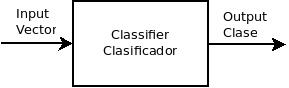
\includegraphics[width=5cm]{diagrams/classifier1.jpg}
	\end{center}
	\caption{Modelo general de un clasificador}
	\label{fig:classif1}
	\end{figure}

En la figura \ref{fig:classif1} se puede apreciar el esquema general de un algoritmo clasificador. Lo que se encuentra en la caja ``clasificador'' es el modelo que va a ser utilizado para clasificar. Uno de los problemas que hay que resolver antes de proceder a la clasificación es encontrar un modelo que pueda aproximar lo mejor posible la realidad del problema que se desea solucionar. Varios autores han especificado que hasta el momento no se ha encontrado un modelo que se ajuste de la mejor manera a todos los problemas, a esto le han llamado {\it ``no free lunch theorem''}, es español esto traduciría ``teorema no hay almuerzo gratis''. En algo si concuerdan la mayoría de investigadores, y es en que si varios modelos funcionan bien se debe escoger el más sencillo de ellos. Esta observación se desprende del principio filosófico conocido como la navaja de Ockham, propuesto por Guillermo de Ockham (1280-1349), según el cual ``cuando dos teorías en igualdad de condiciones tienen las mismas consecuencias, la teoría más simple tiene más probabilidades de ser correcta que la compleja'' \footnote{Robert Audi, ed. Ockham's razor. The Cambridge Dictionary of Philosophy (2nd Edition). Cambridge University Press}. Este principio se aplica en muchos campos, y para el caso del aprendizaje de máquinas tiene especial sentido, ya que usualmente los modelos más sencillos son más fáciles de entrenar, de comprender y sobre todo de depurar.

\subsection{El aprendizaje de máquinas}
\label{sect:machineLearning}

Con los avances en las tecnologías de cómputo la sociedad tiene la posibilidad de almacenar y procesar grandes cantidades de información. Por ejemplo, las cadenas de supermercado poseen grandes volúmenes de información de sus ventas, y las entidades financieras poseen la información crediticia de todos sus clientes. Para los supermercados es muy útil saber que personas compran ciertos tipos de productos y con qué periodicidad, y para las entidades financieras es útil saber que personas son de mayor y menor riesgo crediticio.

Si, por ejemplo, supiéramos con exactitud cómo establecer si una persona es de riesgo o no para una central de crédito dados sus datos financieros, no necesitaríamos utilizar
aprendizaje de máquinas; podríamos simplemente escribir las reglas que determinan si una persona es de riesgo o no y aplicarlas. Pero dado que muchas veces no es posible establecer estas reglas, lo que se busca al realizar aprendizaje de máquinas es extraer esta información de los datos.

Alpaydin indica que las personas usualmente sabemos que existen procesos que explican los datos que observamos. Por ejemplo, en el caso del supermercado, el comportamiento de los clientes no es completamente aleatorio; por tanto, se espera encontrar algunos patrones recurrentes en los datos. Aunque este autor indica que muchas veces no es posible identificar el modelo completamente, usualmente se puede construir una buena aproximación. Este es el nicho de trabajo del aprendizaje de máquinas, pues esta aproximación puede ser útil para encontrar patrones en el problema estudiado o para hacer estimaciones de datos futuros, asumiendo que en el futuro los datos van a comportarse de una manera similar a como se comportaron en el pasado.

\section{Algunos algoritmos de clasificación}

Como se indicó en la sección anterior, no hay ningún algoritmo que sea la mejor elección para todo tipo de problemas. En esta sección se pretende presentar algunos de los algoritmos o modelos de aprendizaje de máquinas, sin ahondar en cada uno de ellos, simplemente expondrá brevemente de que se tratan y cuáles son sus ventajas y desventajas.

\subsection{Árboles de decisión}

Un árbol de decisión es un modelo utilizado principalmente para clasificación. Como su nombre lo indica el modelo sigue una estructura de árbol, donde los nodos no terminales son condiciones sobre las variables de entrada y los nodos terminales, o nodos hoja, son las clases.

	\begin{figure}[htb]
	\begin{center}
	\leavevmode
	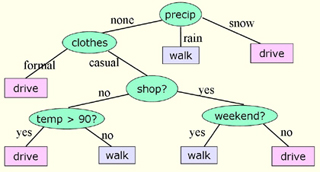
\includegraphics[width=7cm]{img/decisiontree.jpg}
	\end{center}
	\caption{Ejemplo de árbol de decisión, tomado de MIT OpenCourseware.}
	\label{fig:decisionTree}
	\end{figure}

En la figura \ref{fig:decisionTree}, se muestra un ejemplo de un árbol de decisión\footnote{Tomado de ``http://ocw.mit.edu/courses/electrical-engineering-and-computer-science/6-034-artificial-intelligence-spring-2005/'', 12 de Marzo de 2011}. Se puede observar que dependiendo del valor de las variables en cada nodo no terminal se escoge un camino diferente, realizando así un proceso de clasificación por etapas. En ese ejemplo las clases son ``caminar'' y ``conducir''. Es posible examinar el proceso de decisión utilizado para llegar a estas variables. Naturalmente, existen procesos automáticos para generar árboles como el del ejemplo a partir de un conjunto de datos de entrenamiento.

De los árboles de decisión se puede concluir:

	\begin{itemize}
	
	\item Son fácilmente interpretables por un ser humano.

	\item En general son más efectivos en los problemas que tienen entradas discretas.
	
	\item Si el árbol esta balanceado correctamente la velocidad de clasificación es alta.
	
	\item Se debe optimizar la profundidad máxima del árbol, pues un valor adecuado es importante para obtener un buen resultado.
	
	\item El poder clasificatorio de los árboles es limitado, especialmente si se comparan con otros algoritmos de clasificación.
	
	\item La mayoría de algoritmos existentes para generar árboles de decisión solo permiten condiciones sobre una única variable por nodo. En estos casos se limita aun más su poder clasificatorio. 

	\end{itemize}

\subsection{Métodos estadísticos}

La estadística es uno de los métodos más antiguos para inferir el comportamiento de una población a través de una muestra y, sin embargo, todavía está vigente. Se profundizará en este tema en las secciones posteriores, así que por ahora solo se mencionan sus ventajas y desventajas:

	\begin{itemize}

	\item No necesita configuración, lo único que se debe saber en un método estadístico a-priori es la distribución de probabilidad con la que se va a aproximar el modelo real.

	\item Un modelo estadístico es fácil de interpretar por un humano, aunque no es tan fácil de interpretar como los árboles de decisión.

	\item El poder clasificatorio es más alto que el de los árboles de decisión.

	\item Brinda mucha información, en vez de solo determinar a qué clase pertenece una instancia, brida la probabilidad de que la instancia pertenezca cada una de las demás clases.
	
	\end{itemize}
	
\subsection{Redes neuronales artificiales}

Las redes neuronales artificiales son un paradigma de aprendizaje ampliamente tratado en la literatura de la inteligencia artificial.\footnote{ALPAYDIN, Ethem. Introduction to Machine Learning. Estados Unidos: MIT Press, 2004. 415 p.}. Las redes neuronales artificiales (RNA) intentan imitar la naturaleza de la neuronas del cerebro humano. Uno de los modelos más conocidos de redes neuronales son los perceptrones multicapa, cuya estructura se puede apreciar en la figura \ref{fig:rna}.\footnote{Imagen tomada de Wikimedia Commons ``http://upload.wikimedia.org/wikipedia/commons/6/64/RedNeuronalArtificial.png'', 13 de Marzo de 2011)}.

	\begin{figure}[htb]
	\begin{center}
	\leavevmode
	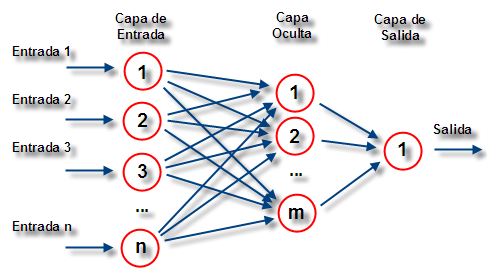
\includegraphics[width=7cm]{img/rna.png}
	\end{center}
	\caption{Ejemplo de un perceptrón con una capa oculta, tomado de Wikimedia}
	\label{fig:rna}
	\end{figure}

Cada neurona tiene una estructura simple. Cada neurona de un perceptrón multicapa recibe un vector de datos de entrada $\vec{x}$, y tiene un vector de pesos sinápticos $\vec{w}$ y una función de activación $f(x)$. Dado sus entradas, la salida $y$ de una neurona es:

\[y = f(\vec{w}.\vec{x})\]

Algunas ventajas y desventajas de las redes neuronales son:

\begin{itemize}

	\item El poder clasificatorio de este método es mayor que el de los métodos anteriormente mencionados. Matemáticamente se ha demostrado que no exigen ninguna distribución determinada de los datos, ni tampoco que estos sean separables linealmente.

	\item Al igual que el método estadístico, con una función de activación adecuada se puede calcular la probabilidad de que una instancia pertenezca a cada clase.

	\item Dada la cantidad de parámetros que se pueden configurar, estos algoritmos son muy difíciles de afinar para un problema determinado.

	\item Las redes neuronales son difíciles de interpretar. Una vez entrenadas pueden dar buenos o malos resultados, pero es difícil saber cuál es el error real, o si es posible mejorar los resultados cambiando los parámetros.

\end{itemize}

\section{Algunos elementos de probabilidad}

Un experimento aleatorio es aquel del cual no se conoce el resultado con certeza\footnote{Ross, S.M. Introduction to Probability and Statistics for Engineers and Scientists. New York: Wiley 1987.}. El conjunto de todos los posibles resultados es llamado espacio muestral $S$, y a cualquier subconjunto de $S$ se le llama evento $E$. Se puede interpretar la probabilidad como una frecuencia: cuando un experimento aleatorio es repetido continuamente bajo las mismas condiciones, la proporción de veces que ocurre en el tiempo el evento $E$ se aproxima a un valor constante; a esto lo denotamos $P(E)$ e indica la probabilidad que el evento $E$ ocurra.

Una variable aleatoria es aquella que puede tomar cualquier valor en distintos experimentos, es decir, su valor no se puede determinar con certeza.

\subsection{Probabilidad condicional y el teorema de Bayes}

La probabilidad condicional es la probabilidad de que un evento $A$ ocurra, dado que se conoce la ocurrencia del evento $B$, y se denota $P(A|B)$. La probabilidad condicional se calcula como:

	\begin{equation}\label{eq:condProb}
		P(A|B) = \frac{P(A \cap B)}{P(B)}
	\end{equation}

Al saber que ocurrió el evento $B$, el espacio muestral se reduce al subconjunto $B$. Dado que la intersección es conmutativa, de la ecuación \ref{eq:condProb} se obtiene:

\[P(A \cap B) = P(A|B)P(B) = P(B|A)P(A)\]

Y con esto se llega al teorema de Bayes:

	\begin{equation}\label{eq:bayes}
		P(A|B) = \frac{P(B|A)P(A)}{P(B)}
	\end{equation}

Cuando el espacio muestral se compone de varios eventos mutuamente exclusivos $A_i$, es decir, $\cup_{i=1}^{n} A_i = S$ entonces:

	\[P(B)=\cup_{i=1}^{n} {A_i \cap B}\]
	
	\begin{equation}\label{eq:bayesDenominator}
		P(B) = \sum_{i=1}^{n}{P(B|A_i)P(A_i)}
	\end{equation}

Entonces, reemplazando la ecuación \ref{eq:bayesDenominator} en la ecuación \ref{eq:bayes}, tenemos:
	
	\begin{equation}\label{eq:bayes2}
		P(A|B) = \frac{P(B|A)P(A)}{\sum_{i=1}^{n}{P(B|A_i)P(A_i)}}
	\end{equation}
	
\subsection{La esperanza matemática}

Supongamos que se realiza un experimento sobre una variable aleatoria $x$ un número infinito de veces, entonces la esperanza de la variable $x$ es el promedio del valor de $x$ en los infinitos experimentos y se denota $E[x]$ (que se lee valor esperado de $x$ o esperanza de $x$). El concepto de esperanza es importante en la probabilidad porque además de tener usualmente un significado de interés para la variable aleatoria estudiada, se espera que independiente de la distribución de probabilidad que sigue la variable $x$, la esperanza de $x$ converja a un valor constante si las condiciones del experimento no cambian. Matemáticamente, el valor de la esperanza de una variable aleatoria $x$ es el siguiente:

	\[ E(X) = \left\{ \begin{array}{ll}
		\sum_{i}{x_iP(x_i)}   & \mbox{si X es una variable discreta} \\
		\int {xp(x)dx} & \mbox{si X es una variable continua}
	\end{array} \right. \]

La esperanza es entonces un promedio ponderado, en donde el peso de cada valor tomado es la probabilidad de que la variable $X$ tome dicho valor. Suponiendo que $X$ y $Y$ son dos variables aleatorias, la esperanza cumpla las siguientes propiedades:

	\[E[aX + b] = aE[X] + b\]
	\[E[X + Y] = E[X] + E[Y]\]

La esperanza de toda función g para la cual $imagen(g) \in \Re$ es:

	\[ E[g(X)] = \left\{ \begin{array}{ll}
		\sum_{i}{g(x_i)P(x_i)}   & \mbox{si X es una variable discreta} \\
		\int {g(x)p(x)dx} & \mbox{si X es una variable continua}
	\end{array} \right. \]

Una función especial se da cuando $g(X) = x^n$:

	\[ E[X^n] = \left\{ \begin{array}{ll}
		\sum_{i}{x_i^nP(x_i)}   & \mbox{si X es una variable discreta} \\
		\int {x^np(x)dx} & \mbox{si X es una variable continua}
	\end{array} \right. \]

Esta función se denomina el enésimo momento de X. El primer momento, por ejemplo, es la media.

\subsection{Desviación estándar, varianza y covarianza}

La varianza mide que tanto varia $X$ alrededor del valor esperado. Si $X$ es una variable aleatoria entonces la varianza se define como el segundo momento menos el cuadrado del primer momento:

	\[Var(X) = E[X^2] - E[X]^2 = E[X^2] - \mu^2\]

La desviación estándar es la raíz cuadrada de la varianza, y como se expresa en las mismas unidades de $X$ es más utilizada que la varianza, pues puede ser interpretada de una manera más fácil. La desviación estándar se denota usualmente con el símbolo $\sigma$.

La covarianza indica la relación que existe entre dos variables aleatorias $X$ y $Y$. Si la ocurrencia de $X$ hace más probable la ocurrencia de $Y$ entonces la covarianza es positiva. Si por el contrario la ocurrencia de $X$ hace menos probable la ocurrencia de $Y$ entonces la covarianza entre ambas es negativa. Si las dos variables no están relacionadas, entonces la covarianza será 0. La covarianza se define matemáticamente como:

	\[Cov(X, Y) = E[XY] - \mu_X\mu_Y\]

\subsection{Distribución de probabilidad}

Una distribución de probabilidad de una variable aleatoria $X$ es una función que asigna una probabilidad a cada posible valor que puede tomar la variable $X$. Cuando $X$ es una variable discreta, la función definirá un valor de probabilidad para cada uno de los valores que $X$ puede tomar. Sin embargo, cuando la variable $X$ es continua, existen infinitos valores posibles que puede tomar y por tanto la probabilidad de obtener un valor especifico es 0. Por esta razón tiene poco sentido hablar de la probabilidad de un valor especifico y la distribución de probabilidad se convierte en una función de distribución, la cual define, para cada real $x$, la probabilidad de que la variable $X$ sea menor o igual a $x$. En esto caso la distribución de probabilidad $D$ se definiría matemáticamente como:

	\[D(x) = P(X \leq x) = \int_{-\infty}^x{f(t)dt}\]

Donde f(t) es una función de densidad continua, que debe ser positiva para todo t, y debe cumplir la propiedad:

	\[\int_{-\infty}^{\infty}{f(t)dt} = 1\]
	
\subsection{La distribución normal}

Muchos fenómenos de la naturaleza siguen una distribución normal, al menos de manera aproximada. Esta distribución tiene forma de campana, lo que significa que los datos se obtienen alrededor de un valor típico con ligeras variaciones. Matemáticamente, si $\mu$ representa el valor típico y $\sigma$ representa cuanto varían las instancias al rededor de este valor típico, la distribución está dada por:

	\begin{equation}
		p(x) = \frac{1}{\sqrt{2\pi}\sigma}exp\left[-\frac{(x-\mu)^2}{2\sigma^2}\right]
	\label{eq:normal}
	\end{equation}

Donde $exp[x]$ es la función exponencial $e^x$, $\mu$ son la media y $\sigma$ se conoce como desviación estándar, que se calculan como se especifica en las secciones anteriores. En una distribución normal el 68.27\% de los datos está entre $(\mu-\sigma, \mu+\sigma)$, el 95.45\% de los datos está entre $(\mu-2\sigma, \mu+2\sigma)$ y el 99.73\% de los datos está entre $(\mu-3\sigma, \mu+3\sigma)$.

\section{La distribución normal multivariable}
\label{sect:multivar}

En muchas ocasiones, en lugar de calcular un único valor $x$ de cada elemento muestreado, se calculan varios valores diferentes generando un vector $\vec{x}$. Supongamos que tenemos un vector d-dimensional $\vec{x}$ que sigue una distribución normal multivariable, entonces:

	\begin{equation}\label{eq:multDens}
		p(x) = \frac{1}{(2\pi)^{d/2}|\Sigma|^\frac{1}{2}} exp\left[{-\frac{1}{2}(\vec{x}-\vec{\mu})\Sigma^{-1}(\vec{x}-\vec{\mu})}\right]
	\end{equation}

Esto se denota como $\vec{x} \sim N(\vec{\mu},\Sigma)$ y significa que $\vec{x}$ sigue una distribución normal multivariable cuya media es el vector $\vec{\mu}$ y cuya matriz de covarianza es la matriz $\Sigma$. Si para cada clase $C_i$ se calculan la media $\vec{\mu_i}$ y la matriz de covarianza $\Sigma_i$, la densidad de probabilidad $p(x|C_i)$ es:

	\begin{equation}\label{eq:multivariate}
		p(x|C_i) = \frac{1}{(2\pi)^{d/2}|\Sigma_i|^\frac{1}{2}} exp\left[{-\frac{1}{2}(\vec{x}-\vec{\mu_i})\Sigma_i^{-1}(\vec{x}-\vec{\mu_i})}\right]
	\end{equation}
	
La distribución normal multivariable puede ser utilizada como un algoritmo de clasificación, pues es un modelo que ha demostrado ser robusto para varias aplicaciones diferentes\footnote{Jerome H. Friedman. Regularized discriminant analysis. Journal of the american statistical association, 84:165–175, 1989.}.	El objetivo es encontrar $P(C_i|x)$, que es la probabilidad posterior de que el vector $\vec{x}$ pertenezca a la clase $C_i$. Si se calcula $P(C_i|x)$ para cada clase $i$, se escoge como la clase correcta la que posea la probabilidad posterior más alta.

Es importante notar que en lugar de simplemente determinar a qué clase pertenece la instancia dada se están calculando también las probabilidades de que pertenezca a cada una de las otras clases, lo que permite calcular el porcentaje de seguridad con el cual el algoritmo está dando su respuesta. Esto es una gran ventaja para el problema de reconocimiento óptico de caracteres, ya que algunas correcciones pueden realizarse en etapas posteriores, por ejemplo, utilizando un diccionario.

Como se puede observar en la ecuación \eqref{eq:multivariate} lo que permite calcular la distribución normal multivariable es $p(x|C_i)$, que es la densidad de probabilidad de la variable aleatoria $\vec{x}$ dada la clase $C_i$; lo que se desea calcular, en cambio, es la probabilidad de que un $\vec{x}$ dado pertenezca a la clase $C_i$, es decir, la probabilidad posterior $P(C_i|\vec{x})$. Para eso se utiliza el teorema de Bayes (ecuación \ref{eq:bayes2}), con el cual la probabilidad posterior se calcula como:

	\begin{equation}\label{eq:multBayes}
		P(C_i|\vec{x}) = \frac{p(\vec{x}|C_i)P(C_i)}{p(x)} = \frac{p(\vec{x}|C_i)P(C_i)}{ \sum_j{p(\vec{x}|C_j)P(C_j)} }
	\end{equation}
	
De la ecuación \ref{eq:multBayes} se puede deducir que $\sum_i{P(C_i|\vec{x})}=1$, y por tanto que $0 \le P(C_i|\vec{x}) \le 1$ para todas las clases.
	
\subsection{Entrenamiento}

Ya se ha visto como se puede llevar a cabo la clasificación una vez que los parámetros $\vec{\mu_i}$ y $\Sigma_i$ han sido calculados para cada clase $C_i$. El entrenamiento consiste entonces en calcular los parámetros $\vec{\mu_i}$ y $\Sigma_i$ a partir de un conjunto de datos de entrenamiento $T$. Primero, el conjunto de entrenamiento se parte en diferentes conjuntos de entrenamiento $T_i$, donde cada conjunto $T_i$ contiene solamente instancias de la clase $C_i$. Entonces, los parámetros se calculan a partir de las ecuaciones:

	\begin{equation}\label{eq:multiParams}
	\begin{aligned}
		\vec{\mu_i} &= E[ \vec{x_i} ] \\
		\Sigma_i(a,b) &= E[ (\vec{x_i}-\vec{\mu_a})(\vec{x_i}-\vec{\mu_b}) ]
	\end{aligned}
	\end{equation}

Donde $\vec{x_i}$ son las instancias del conjunto $T_i$, $E[x]$ es el valor esperado o media de $x$ y $\Sigma_i(a,b)$ es el valor en la fila $a$ y la columna $b$ de la matriz $\Sigma_i$.

\subsection{Simplificaciones de la distribución normal multivariable}

Dado que la matriz de covarianza es de tamaño $d \times d$, el número de parámetros de la distribución normal multivariable crece cuadráticamente con el número de dimensiones $d$. Esto se convierte en un problema cuando no hay suficientes datos para estimar los parámetros de manera apropiada\footnote{Wald and Kornmal. Discriminant functions when covariances are unequal and sample sizes are moderate. Biometrics, 33:479–484, 1977.}. Supongamos que de una muestra de tres instancias se desea calcular la media y la varianza de la población. Es claro que aunque los parámetros pueden ser calculados, probablemente no representarán bien los parámetros de la población. De la misma manera, cuantos más parámetros se deban calcular se necesita una mayor cantidad de datos para obtener una mejor generalización.

Una manera de realizar las clasificación es calcular la distancia Mahalanobis entre la entrada y la media de cada clase, y escoger la que tenga la menor distancia. La distancia Mahalanobis $d_i$ entre la entrada $\vec{x}$ y la clase $C_i$, está dada por:

	\begin{equation}
		\label{eq:mahalanobis}
		d_i = (\vec{x}-\vec{\mu_i})\Sigma(\vec{x}-\vec{\mu_i}) 
	\end{equation}

Cuando la matriz de covarianza es igual a la matriz identidad la distancia Mahalanobis se convierte en la distancia euclidiana al cuadrado, pero en los demás casos puede proporcionar valores mucho más adecuados para calcular la cercanía de una entrada a cada una de las clases. En el caso de una distribución normal multivariable, es posible utilizar una matriz de covarianza compartida por todas las clases para calcular la distancia Mahalanobis. Las probabilidades posteriores pueden ser calculadas de la misma manera, y se sigue escogiendo la clase con mayor probabilidad posterior.

%Quedó faltando la distribución normal multivariable con matriz de covarianza semi-compartida

\chapter{Extracción de características de los caracteres}
\label{chap:features}

\section{Introducción}

Como se explicó en la sección \ref{sect:machineLearning}, para hacer aprendizaje de maquinas es necesario primero obtener unas características que permitan diferenciar entre las distintas clases. En el caso del reconocimiento óptico de caracteres se requieren características que permitan diferenciar, por ejemplo, el número '5' del número '8'. Para obtener estas características se requieren realizar algunas etapas de procesamiento que detecten donde están los caracteres y que forma tienen. En las siguientes secciones se describirán las etapas de procesamiento que se realizaron en este proyecto.

\section{Escala de grises}

Antes de computar las características es necesario hacer un preprocesamiento. Primero la imagen debe convertirse a un formato más apropiado para extraerle las características. Dado que las letras no varían con el color, y que el objetivo del sistema no es reconocer colores, es conveniente convertir la imagen a una escala de grises. En este proyecto se trabajo con el modelo RGB. En este modelo se asigna una intensidad a cada uno de los tres colores primarios de la luz: rojo, verde y azul\footnote{que en ingles son red, green, y blue, de allí las iníciales RGB}, de esta manera cada píxel en una fotografía se representa mediante un valor que identifique la intensidad de cada uno de estos tres colores que, mezclados por adición, se acerque más al color verdadero del píxel. Las cámaras digitales modernas utilizan valores entre\footnote{en donde 0 representa que el color no se utiliza y 255 representa la mayor intensidad} 0 y 255 ($2^8$) permitiendo de esta manera más de 16 millones de colores distintos. En una escala de grises, en cambio, cada píxel es representado con un único valor entre 0 y 255, el cual representa que tan oscuro es el mismo. Para convertir un píxel de una imagen en color a uno en escala de grises se suele hacer un promedio ponderado de la intensidad de cada uno de los tres colores, en donde a cada color se le asigna un peso. Al ser un promedio ponderado la suma de los tres pesos debe ser igual a 1. Los pesos utilizados más comúnmente son:

\begin{equation}\label{eq:bwtocv}
	gris = 0.2989 * rojo + 0.5870 * verde + 0.1140 * azul 
\end{equation}

Estos pesos se utilizan en la librería de visión computador OpenCV\footnote{tomado de $http://opencv.willowgarage.com/documentation/c/miscellaneous_image_transformations.html$, abril 4 de 2011} y fueron calculados a partir de observaciones de la sensibilidad del ojo humano a cada uno de los tres colores. 

Haciendo uso de la ecuación \ref{eq:bwtocv} se implementó un algoritmo para obtener una imagen en escala de grises a partir de una imagen RGB. 

\section{Binarización}
\label{sect:binarization}

Una vez obtenida la imagen en escala de grises se procedió a hacer una binarización. La binarización es un proceso que transforma una imagen en escala de grises a una imagen en dos colores: blanco o negro. Esto es útil para el reconocimiento de caracteres debido a que las letras y los dígitos en escala de grises no se distinguen por la intensidad de los píxeles que los componen sino por la forma que estos producen. De esta manera, al convertir las imágenes a blanco y negro se pierde muy poca información relevante y se simplifica la representación de cada píxel, pasando de 256 posibles valores a tan solo 2. Un método muy utilizado para binarizar una imagen es escoger un valor umbral $T(x,y)$ para cada píxel $(x,y)$ y establecer el valor de cada píxel como:

\begin{equation}\label{binEq}
	I_2(x,y) = \left\{ \begin{array}{ll}
		0   & \mbox{si $I_1(x,y) < T(x,y)$} \\
		255 & \mbox{en cualquier otro caso}
	\end{array} \right. 
\end{equation}

Donde $I_1(x,y)$ es la imagen original y $I_2(x,y)$ es la imagen binarizada. Usualmente, la diferencia entre los distintos métodos de binarización se encuentra en como elige cada uno el valor umbral $T(x,y)$.

Cuando las imágenes son adquiridas mediante un escáner, es común escoger un $T(x,y)$ constante para todos los píxeles. Esto es debido a que en una imagen escaneada se logra una iluminación aproximadamente constante en todo el documento. Como en este caso la imagen es adquirida utilizando una cámara digital, en condiciones de iluminación no tan constantes, se decidió elegir un método de binarización local adaptativo. En un método de este tipo $T(x,y)$ puede ser distinto para cada píxel, y se dice que es local porque $T(x,y)$ se calcula utilizando información sobre el vecindario de píxeles del píxel $(x,y)$. Uno de los métodos que ha dado los mejores resultados\footnote{De hecho es el que se utiliza en varios OCRs libres.} para el reconocimiento de caracteres es el de Sauvola, en el cual $T(x,y)$ se obtiene utilizando la siguiente ecuación:

\begin{equation}\label{rSauvola}
	T(x,y)=m(x,y)\left[ 1 + k(\frac{s(x,y)}{R}-1) \right]
\end{equation}

Donde $m(x,y)$ es la media y $s(x,y)$ la desviación estándar de los píxeles en algún área alrededor de $(x,y)$, y R es el máximo valor de la desviación estándar (128 para una imagen en escala de grises). La forma más sencilla de implementar este algoritmo es calcular para cada píxel $(x,y)$ el valor de $m$ y $s$ de manera directa, es decir, iterar por todos los píxeles en el vecindario de $(x,y)$. Sin embargo, si el área a considerar para $m$ y $s$ es de tamaño $A \times A$, entonces la complejidad computacional de calcular $T(x,y)$ para todos los píxeles de una imagen de tamaño $N \times M$ sería $O(N \times M \times A^{2})$\footnote{La función $O(f)$ se usa para indicar que la complejidad algorítmica es una función $f(N)$ que depende de la talla del problema $N$. Sea $T(N)$ el tiempo de  ejecución del algoritmo para una talla de problema $N$, entonces existe una constante $K$ tal que  $\forall N ( K*f(N) < T(N) ) $}. Con esta complejidad el algoritmo sería demasiado lento para procesar imágenes de varios mega píxeles, incluso con valores relativamente pequeños de $A$.

\subsection{Optimización al algoritmo de binarización}

Dada la complejidad del algoritmo estándar de binarización, se hizo una investigación para buscar algoritmos ya existentes que realizaran la tarea en un tiempo más razonable. En un artículo escrito por los creadores del proyecto Ocropus\footnote{Un proyecto de código abierto cuyo objetivo es crear un sistema de reconocimiento óptico de caracteres} se propone\footnote{Efficient Implementation of Local Adaptive Thresholding Techniques Using Integral Images} un algoritmo que binariza una imagen en un tiempo $O(N \times M)$ utilizando imágenes integrales y el método de Sauvola. Una imagen integral se define para un píxel $(x, y)$ como la suma de todos los píxeles por encima y a la izquierda de este píxel. Matemáticamente la imagen integral del píxel $(x, y)$ se puede definir como:

\begin{equation}
	I(x, y) = \sum_{i=0}^{x}\sum_{j=0}^{y}Im(i, j)
\end{equation}

Donde $Im(i, j)$ es el valor del píxel ubicado en la posición $(i, j)$. Dado que es posible obtener la imagen integral de una imagen en tiempo $O(N \times M)$, los autores indicaron que es posible calcular el valor de la media $m$ del área $A^{2}$ alrededor del píxel $(x, y)$ en un tiempo constante de la siguiente forma:

\begin{align*}
  m(x, y) =& (I(x + \frac{A}{2}, y + \frac{A}{2}) + I(x - \frac{A}{2}, y - \frac{A}{2}) \\
	   &- I(x + \frac{A}{2}, y - \frac{A}{2}) - I(x - \frac{A}{2}, y + \frac{A}{2})) / A^{2}
\end{align*}

\begin{figure}[htb]
\begin{center}
\leavevmode
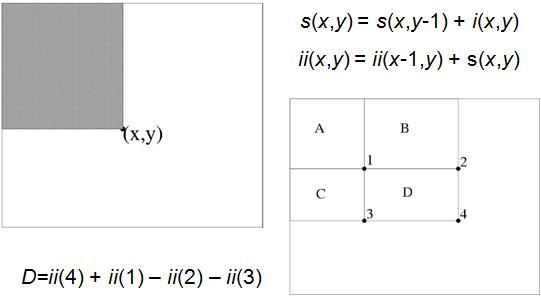
\includegraphics[width=6cm]{img/integral.png}
\end{center}
\caption{Imagen integral (Tomado de ACM Student Reseach Competition)}
\label{fig:integral}
\end{figure}

En el cuadrado de tamaño $A \times A$ alrededor del píxel $(x, y)$, esto equivale simplemente a sumar los valores de la imagen integral en el píxel de más abajo a la derecha y en el píxel de más arriba a la izquierda, y restar los valores de la imagen integral en el píxel de más abajo a la izquierda y en el píxel de más arriba a la derecha. La representación gráfica de las imágenes integrales se puede apreciar en la figura \ref{fig:integral}\footnote{Xu Liu. ``Mobile Currency Reader for People with Visual Impairments''. ACM Student research competition}. La fórmula para hallar la desviación estándar no es presentada en el artículo de los creadores de Ocropus, y solo se menciona que se puede calcular utilizando la imagen integral de los píxeles al cuadrado. Con esta pista es fácil deducir matemáticamente la fórmula para calcular la desviación estándar:

\[ \sigma^2 = \frac{1}{w^2}\left(\sum_w{p(x,y)^2} - \mu \sum_w{p(x,y)}\right) \]

El resultado obtenido es consistente con la formula que se utilizo en la implementación de dicho algoritmo en el proyecto Ocropus\footnote{Ocropus es un software de OCR libre desarrollado por Google, esta licenciado bajo Apache Licence 2.0}.

Posteriormente se implemento el algoritmo. Ya que era una de las partes de mayor complejidad algorítmica en el sistema, se implemento de la manera más eficiente posible, utilizando las recomendaciones del libro oficial de OpenCV. En especial se utilizaron punteros en donde fuera posible en vez de contadores, reemplazando la matriz por un único arreglo, el cual se accedió a través de un único puntero. Es decir, para acceder a cada posición en una matriz normalmente se requiere multiplicar la fila actual por el tamaño de cada fila, a esto sumarle la posición de la columna actual, multiplicar todo esto por el tamaño de cada elemento dentro del arreglo, y finalmente sumarle este valor al puntero base de la matriz. De la forma en que se implemento, en cada iteración únicamente era necesario sumarle el tamaño de cada elemento al puntero. La función resultante realiza la binarización 7 veces más rápido que la función utilizada en el proyecto Ocropus, ya que se prefirió darle mayor importancia a la eficiencia, pues en un futuro esta función podría utilizarse para binarizar imágenes en un dispositivo móvil con una capacidad de procesamiento limitada. El resultado del algoritmo implementando sobre una imagen se muestra en la figura \ref{fig:binarization}, la figura \ref{fig:bin1} muestra la imagen original y la figura \ref{fig:bin2} muestra la misma imagen después de aplicarle el algoritmo de binarización implementado.

	\begin{figure}
	\centering
		\subfloat[Antes de binarizar]{\label{fig:bin1}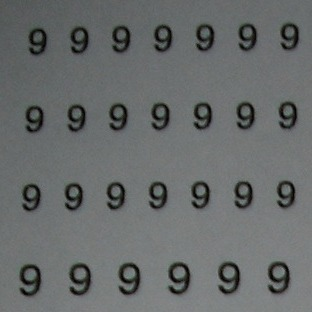
\includegraphics[width=4cm]{img/bin1.jpg}}
		\subfloat[Después de binarizar]{\label{fig:bin2}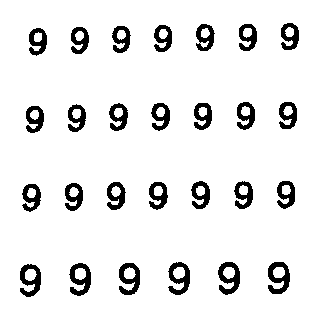
\includegraphics[width=4cm]{img/bin2.png}}
	\caption{Figuras antes y después de la binarización}
	\label{fig:binarization}
	\end{figure}


\section{Componentes conectados}
\label{sect:conComponents}

Antes de reconocer los caracteres es necesario saber en qué partes de la imagen se encuentran ubicados. Para encontrarlos es necesario agrupar los píxeles de tal forma que todos los puntos pertenecientes a un caracter queden en un mismo grupo. Si asumimos que $I_2(x,y)$ es la imagen binarizada resultante de aplicar el método de Sauvola de la ecuación \eqref{rSauvola} en la ecuación \eqref{binEq}, entonces podemos definir que un píxel $(x,y)$ pertenece al fondo de la imagen si $I_2(x,y)=255$, y pertenece a algún caracter si $I_2(x,y)=0$. Si se establece que un píxel $(x',y')$ es vecino de un píxel $(x,y)$ si $|x-x'|=1$ y $|y-y'|=1$ entonces se puede definir un componente conectado como un conjunto de píxeles $C=\{(x_i,y_i)\}$ en donde $\forall{(x_i,y_i)}, I_2(x_i,y_i)=0$ y para cada $i,j$ existe un camino entre $(x_i,y_i)$ y $(x_j,y_j)$ moviéndose únicamente a través de píxeles vecinos de $C$. La idea de los componentes conectados fue utilizada, entre muchos otros, por O'Gorman\footnote{O’GORMAN Lawrence. The Document Spectrum for Page Layout Analysis.} para realizar el análisis del documento, una de las etapas del reconocimiento óptico de caracteres.

\newtheorem{pixHasOneC}{Lemma}
\begin{pixHasOneC}
	Cada píxel $(x,y)$ tal que $I_2(x,y)=0$ pertenece a un único componente conectado.
\end{pixHasOneC}
\begin{proof}
	Suponga que un píxel $(x,y)$ pertenece a más de un componente conectado. En particular, suponga que $(x,y)$ pertenece tanto al componente $C_i$ como al componente $C_j$. Entonces hay un camino desde cualquier $P_i \in C_i$ a $(x,y)$ y desde cualquier $P_j \in C_j$ a $(x,y)$. Por tanto hay al menos un camino desde todo $P_i$ a todo $P_j$, este camino es $P_i \rightarrow (x,y) \rightarrow P_j$. Esto significa que $C_i$ y $C_j$ pueden ser unidos en un único componente conectado, y al unirlos $(x,y)$ pertenecería a un único componente conectado.
\end{proof}

Después de esto se puede utilizar un algoritmo de relleno por difusión ({\em flood-fill}) para encontrar cada componente conectado. Dado un píxel $(x,y)$ con $I_2(x,y)=0$, se encuentra el componente conectado al que este pertenece, se guarda, y se borra de la imagen. De esta manera por cada píxel encontrado en un único recorrido por toda la imagen se extraerá un componente conectado, y al finalizar este recorrido se habrán extraído todos los componentes conectados. Este algoritmo se implementó utilizando una pila para evitar la recursividad.

	\begin{figure}
	\centering
		\subfloat{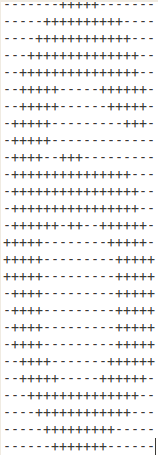
\includegraphics[width=2cm]{img/p1.png}}
		\hspace{1cm}
		\subfloat{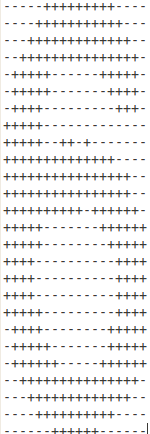
\includegraphics[width=2cm]{img/p2.png}}\\		
	\caption{Componentes conectados extraídos por la aplicación}
	\label{fig:concomp}
	\end{figure}
	
La figura \ref{fig:concomp} muestra dos componentes conectados extraídos por la aplicación implementada de la misma imagen. Observe a pesar de estar en la misma imagen, ser del mismo tamaño y de la misma clase (Dígito '6'), ambas instancias son ligeramente diferentes.

\section{Extracción de características}

Como se explicó en el capítulo \ref{chap:ml}, los métodos de clasificación necesitan unas características de entrada que permitan diferenciar los objetos a clasificar. En el caso específico de los métodos estadísticos, se necesitan vectores de números reales que sean similares para el mismo caracter independiente de el tamaño o inclinación que tenga en caracter en cuestión. Si las imágenes fueran adquiridas mediante un escáner, la inclinación podría ser muy pequeña, incluso tanto que podría despreciarse. Sin embargo, cuando las imágenes son adquiridas mediante una cámara digital, la inclinación entra a ser un factor importante, más aun cuando quien las obtiene es una persona invidente. Por estas razones es necesario encontrar características que sean invariantes a la rotación y al escalamiento, es decir, que al rotar o escalar un mismo caracter el valor numérico de las características sea similar. Dado que la entrada del método estadístico es un vector, esta similitud se puede expresar en términos vectoriales como una distancia Mahalanobis (ecuación \ref{eq:mahalanobis}) relativamente pequeña entre el vector de características de la imagen original y de la imagen rotada.

Para lograr un cierto grado de independencia de las características a la rotación y al escalamiento se pueden tomar dos enfoques: un primer enfoque es transformar la imagen, esto significa rotarla y escalarla para hacerla lo mas similar posible a un patrón estándar, después de esto se pueden extraer características numéricas de la imagen que sean lo más similares posibles para objetos de la misma clase y lo mas diferentes posibles para objetos de distintas clases. Un segundo enfoque consiste en trabajar la imagen tal cual es tomada por la cámara, y utilizar características en las que se obtengan valores numéricos similares para una misma imagen rotada y escalada, es decir, que sean invariantes a la rotación y el escalamiento.

\subsection{Rotación y escalamiento mediante transformación geométrica}
\label{sect:rotation}

Si se utilizan características dependientes a la rotación, se debe entrenar el clasificador con distintas instancias que tengan distintos ángulos de rotación. Si se hace difícil obtener ejemplos reales, una opción puede ser construir ejemplos virtuales\footnote{Niyogi, P. and Girosi, F. and Poggio, T. Incorporating prior information in machine learning by creating virtual examples}. El problema con este enfoque es que tiene una alta complejidad computacional y que instancias de una misma clase pueden quedar ampliamente repartidas por el híper-espacio de clasificación. Como resultado sería más difícil para un algoritmo de clasificación separar las distintas clases.

Un enfoque mucho más práctico es detectar la rotación y el escalamiento del texto, y posteriormente aplicar transformaciones geométricas para ajustar la rotación y el escalamiento a valores preestablecidos. Después de esto se podrían obtener características dependientes a la rotación y al escalamiento para clasificar cada letra. Para detectar la rotación se pueden utilizar métodos ya existentes, como los utilizados en el algoritmo de análisis de documentos Docstrum\footnote{O'GORMAN Lawrence. The Document Spectrum for Page Layout Analysis}, los cuales permiten establecer cuál es la inclinación de cada línea de texto. Al tener la inclinación de las líneas, se puede aproximar cual es la inclinación da cada caracter en particular. Para corregir la inclinación se utilizaría una matriz de rotación: si el algoritmo de detección de rotación determina que el caracter está rotado un ángulo $\theta$ alrededor de su centroide, se puede detectar cual es la nueva ubicación $(x', y')$ del píxel $(x, y)$ utilizando la siguiente operación:

	\[
		\begin{pmatrix} 
			x' \\ y'
		\end{pmatrix}
		=
		\begin{pmatrix} 
			\cos\theta & -\sin\theta \\
			\sin\theta & \cos\theta
		\end{pmatrix}
		\begin{pmatrix} 
			x \\ y
		\end{pmatrix}
	\]

El escalamiento se podría ajustar haciendo una interpolación de los píxeles al tamaño deseado. Existen, sin embargo, dos problemas con esta solución. En cuanto a la rotación, si el ángulo $\theta$ no es un múltiplo de 90 grados, las coordenadas de los nuevos píxeles $(x', y')$ no serían enteras. Esto se puede solucionar interpolando $(x',y')$ a sus vecinos enteros más cercanos, pero este proceso conlleva una pérdida de información importante cuando la calidad de las imágenes no es muy buena. En cuanto al escalamiento, la interpolación también produce una pérdida de información. Tal vez el problema más grave de esta pérdida de información en el reconocimiento de caracteres, es que en algunos casos se puede partir un único caracter en varias partes, dificultando el proceso de reconocimiento.

Para el problema de reconocimiento de caracteres es entonces conveniente encontrar métodos de extracción de características que minimicen la pérdida de información, pero que al mismo tiempo sean invariantes a la rotación y al escalamiento. Los momentos invariantes son características que cumplen dicha propiedad.

\subsection{Momentos invariantes de Hu}	
\label{sect:invariants}

Los momentos invariantes fueron propuestos por primera vez por Hu\footnote{M.K Hu. Visual pattern recognition by moment invariants}. Estos momentos pueden ser considerados como un promedio ponderado de los píxeles de una imagen. Hu computo sus invariantes utilizando los momentos geométricos, los cuales son variantes a la rotación y al escalamiento. Los momentos geométricos se definen como:

	\begin{equation}\label{eq1}
		\mu_{pq} = \iint{ {(x-\bar{x})^p} {(y-\bar{y})^q} f(x,y) dy dx }
	\end{equation}

Donde $\mu_{pq}$ es el momento geométrico de orden $(p+q)$, $f(x,y)$ es el valor del píxel en la posición $(x,y)$ de la imagen y $(\bar{x},\bar{y})$ es el centroide de la misma. Partiendo de estos momentos podemos obtener $n_{pq}$, un momento de orden $(p+q)$ que es invariante al escalamiento:

	\begin{equation}\label{eq2}
		n_{pq} = \frac{\mu_{pq}}{ \mu_{00}^{1+\frac{p+q}{2}} }
	\end{equation}

Utilizando $n_{pq}$, Hu logro un conjunto de momentos invariantes, todos con un grado menor o igual a 3. Sus siete momentos invariantes son:

	\begin{align}
		\phi_1 =& n_{20} + n_{02}, \notag\\ 
		\phi_2 =& (n_{20} - n_{02})^{2} + 4n_{11}^{2}, \notag \\ 
		\phi_3 =& (n_{30} - 3n_{12})^{2} + (3n_{21} - n_{03})^{2}, \notag \\ 
		\phi_4 =& (n_{30} + n_{12})^{2} + (n_{21} + n_{03})^{2},\notag \\ 
		\phi_5 =& (n_{30} - 3n_{12})(n_{30} + n_{12})((n_{30} + n_{12})^{2} \notag \\
				& - 3(n_{21} + n_{03})^{2}) + (3n_{21} - n_{03})(n_{21} + n_{03})\notag\\ 
				& \times (3(n_{30} + n_{12})^{2} - (n_{21} + n_{03})^{2}),\notag\\ 
		\phi_6 =& (n_{20} - n_{02})((n_{30} + n_{12})^{2} - (n_{21} + n_{03})^{2})\notag\\
				& + 4n_{11}(n_{30} + n_{12})(n_{21} + n_{03}),\notag\\
		\phi_7 =& (3n_{21} - n_{03})(n_{30} + n_{12})((n_{30} + n_{12})^{2}\notag\\
				& - 3(n_{21} + n_{03})^{2}) - (n_{30} - 3n_{12})(n_{21} + n_{03}) \notag\\
				& \times (3(n_{30} + n_{12})^{2} - (n_{21} + n_{03})^{2}) \label{eq:huMom} \\ \notag
	\end{align}

\subsection{Momentos complejos y momentos de Fluzzer}

En 1984 Mostafa y Psaltis \cite{mostaf84} propusieron los momentos complejos como una forma alternativa de lograr momentos invariantes. Un momento complejo $C_{pq}$ de orden $(p+q)$ para una imagen $f(x,y)$ se define como:

	\[ C_{pq} = \iint{ (x+iy)^p (x-iy)^q f(x,y) dx dy } \]
	
Donde i denota la unidad imaginaria. En coordenadas polares esto es equivalente a:

	\begin{equation}\label{eq:polarCplx}
		C_{pq} = \iint{ r^{p+q+1}e^{i(p-q)\theta}f(r,\theta) dr d\theta }
	\end{equation}

Una propiedad interesante de los momentos complejos, que se deriva de la ecuación \ref{eq:polarCplx}, es que, si hay una imagen $f'(r,\theta)$ que es una versión rotada un ángulo $\alpha$ sobre el origen de la imagen $f(r,\theta)$, es decir, que $f'(r,\theta) = f(r,\theta+\alpha)$ entonces:

\begin{equation}\label{eq:rotProp}
	C'_{pq} = e^{-i(p-q)\alpha}C_{pq}
\end{equation}

Donde $C'_{pq}$ es el momento complejo de $f'(r,\theta)$ y $C_{pq}$ es el momento complejo de $f(r,\theta)$. Flusser noto\cite{flusser99} que aun cuando se puede probar de la ecuación \ref{eq:rotProp} que $|C_{pq}|$ es invariable a la rotación, estos momentos no generan un conjunto completo de invariantes. Flusser también demostró que los momentos de Hu no eran ni completos ni independientes, y propuso un método para generar un conjunto completo de momentos invariantes de orden arbitrario. Cuando este método se utiliza para generar momentos de grado menor o igual a cuatro, se obtienen 11 momentos invariantes.

\section{Primeros resultados}
\label{sect:exp}

Para el primer experimento se implementó un método de clasificación estadístico multivariable y se implementaron las características de Hu y de Flusser como se indica en el capítulo de diseño, implementación y pruebas del aplicativo. Después de haber corregido los errores encontrados en la etapa de pruebas se obtuvieron los resultados que se muestran en la tabla \ref{tb:exp1_1}.

	\begin{table}
	\begin{center}
	\begin{tabular}{|c|>{\centering\arraybackslash}m{3cm}|>{\centering\arraybackslash}m{3cm}|}
		\hline
		* & \multicolumn{2}{|c|}{Matriz de covarianza independiente} \\
		\hline
		Caracter & Hu & Flusser \\
		\hline
		0 & 99.86\% & 100.00\% \\
		1 & 100.00\% & 100.00\% \\
		2 & 91.21\% & 93.91\% \\
		3 & 100.00\% & 100.00\% \\
		4 & 100.00\% & 96.41\% \\		
		5 & 26.95\% & 38.95\% \\ 
		6 & 93.61\% & 86.83\% \\
		7 & 100.00\% & 99.87\% \\
		8 & 96.76\% & 99.44\% \\
		9 & 65.40\% & 65.03\% \\
		\hline
		Total & 87.21\% & 87.84\% \\
		\hline
	\end{tabular}
	\end{center}
	\caption{Precisión del algoritmo clasificador en el primer experimento}	
	\label{tb:exp1_1}
	\end{table}

Los porcentajes para algunos de los dígitos fueron inusualmente bajos con relación a lo que se esperaba. Si bien se esperaba que los dígitos que presentan cierta simetría, como el 0 y el 8, tuvieran porcentajes de reconocimiento menor, lo que sucedió en realidad fue que tuvieron un porcentaje muy alto, mientras que otros como el 2 y el 5 tuvieron porcentajes muy bajos. Dado que el 6 y el 9 son completamente simétricos respecto a la rotación los resultados fueron cercanos a lo esperado, con la excepción de que el 6 tuvo un porcentaje bastante alto.

Dado los problemas antes mencionados, se decidió indagar las razones por las que algunos dígitos tenían porcentajes muy bajos. En el proceso de depuración se descubrió que el determinante de la matriz de covarianza era muy cercano a cero (con cifras cercanas a $10^{-40}$), por lo cual era muy probable que ciertos cálculos con números de punto flotante tuvieran pérdidas importantes de precisión. Se estudio la posibilidad de utilizar aritmética de precisión arbitraria, sin embargo, dada la complejidad algorítmica, se concluyo que el uso de aritmética implementada en software haría demasiado lento el proceso de reconocimiento.

Otra posibilidad que se exploro fue encontrar matemáticamente una manera en la cual los cálculos pudieran realizarse sin perder mucha precisión, para lo cual se partió de la ecuación de la distribución normal multivariable:

	\[p(x|C_i) = \frac{1}{(2\pi)^{d/2}|\Sigma_i|^\frac{1}{2}} exp\left[{-\frac{1}{2}(\vec{x}-\vec{\mu_i})\Sigma_i^{-1}(\vec{x}-\vec{\mu_i})}\right]\]

Como puede observarse, el determinante de la matriz de covarianza afecta al resultado en dos partes de la misma: hace parte del denominador y del exponente. Dado que para el cálculo de la distancia Mahalanobis se había calculado la matriz de covarianza compartida para todas las clases, se decidió reemplazar el valor de su determinante (que era mucho mayor) por el determinante de la matriz de covarianza. Esto se decidió dado que matemáticamente el valor tiene un significado similar, y por cuanto se considero que los resultados con el valor tan pequeño que se estaba utilizando podían tener poco sentido. Matemáticamente la función fue modificada de la siguiente forma:

	\begin{equation}\label{eq:semishared}
		p(x|C_i) = \frac{1}{(2\pi)^{d/2}|\Sigma|^\frac{1}{2}} e^{-\frac{1}{2}(\vec{x}-\vec{\mu_i})\Sigma_i^{-1}(\vec{x}-\vec{\mu_i})}
	\end{equation} 

Es decir, lo que se hizo fue una mezcla entre el método completo de distribución normal multivariable y un modelo con matriz de covarianza compartida. Los resultados mejoraron significativamente como se esperaba, el resultado se puede apreciar en la tabla \ref{tb:exp1_2}.

	\begin{table}
	\begin{center}
	\begin{tabular}{|c|>{\centering\arraybackslash}m{3cm}|>{\centering\arraybackslash}m{3cm}|}
		\hline
		* & \multicolumn{2}{|c|}{Matriz de covarianza semi-compartida} \\
		\hline
		Caracter & Hu & Flusser \\
		\hline
		0 & 99.34\% & 99.21\% \\
		1 & 100.00\% & 100.00\% \\
		2 & 100.00\% & 100.00\% \\
		3 & 100.00\% & 100.00\% \\
		4 & 100.00\% & 100.00\% \\		
		5 & 97.97\% & 99.32\% \\ 
		6 & 91.65\% & 86.96\% \\
		7 & 100.00\% & 100.00\% \\
		8 & 85.53\% & 92.97\% \\
		9 & 89.52\% & 81.06\% \\
		\hline
		Total & 96.38\% & 95.83\% \\
		\hline
	\end{tabular}
	\end{center}
	\caption{Precisión del algoritmo clasificador en el segundo experimento}	
	\label{tb:exp1_2}
	\end{table}

	\begin{table}
	\begin{center}
	\begin{tabular}{|c|c|c|}		
		\hline
		Experimento & Matriz de covarianza semi-compartida & Matriz de covarianza independiente \\
		\hline
		1 & 96.38\% & 87.84\% \\
		2 & 98.77\% & 92.47\% \\
		\hline		
	\end{tabular}
	\end{center}
	\caption{Comparación de los métodos estadísticos en el problema de OCR}	
	\label{tb:classifResult}
	\end{table}

De las anterior tablas se puede concluir que esta mezcla puede dar buenos resultados cuando el determinante de la matriz de covarianza normal sea muy cercano a cero. La única diferencia entre la ecuación de la distribución normal multivariable y la ecuación modificada (\ref{eq:semishared}) es que la matriz de covarianza en el coeficiente es compartida para todas las clases $\Sigma$; pero la matriz de covarianza en el exponente $\Sigma_i$ sigue siendo diferente para todas las clases (no es compartida).

Dado que no se encontró descrito en la literatura científica, a este método se le denominará ``distribución normal multivariable con matriz de covarianza semi-compartida''.

\subsection{Problemas de simetría mutua}
\label{sect:mutualSym}

Si se analizan los resultados de la tabla \ref{tb:exp1_2} para el método de clasificación de matriz de covarianza semi-compartida se puede observar que el peor porcentaje se obtuvo en los dígitos 6 y 9. De hecho, se noto que estos dígitos se estaban confundiendo entre ellos.
 
Cabe recordar que las características son invariantes a la rotación. Una situación en donde los seres humanos hacen reconocimiento de dígitos con características invariantes a la rotación ocurre cuando juegan billar y deben reconocer los dígitos marcados en las bolas de billar independientemente de la rotación de la bola. En este caso incluso los seres humanos tenemos problemas para reconocer entre la bola 6 y la 9, y necesitamos de una seña (que puede ser una raya) para reconocer entre estos dos dígitos de manera apropiada.

En este caso, el problema no estaba previsto y solo se detectó cuando se realizaron las pruebas. Lo que sucede es que los dígitos 6 y 9 tienen simetría mutua, y son difíciles de reconocer entre ellos por cuanto en los documentos impresos no se hacen señas como en el billar. Sin embargo, cabe recordar que en los objetivos se restringió a que los documentos analizados tendrían una rotación entre $-30^\circ$ y $30^\circ$. Si el documento tuviese un ángulo de rotación por fuera de este rango, se podría llevar a un rango cercano rotando la imagen en múltiplos de $90^\circ$ sin ninguna pérdida de información (ver sección \ref{sect:rotation}), esto, si se cuenta con alguna referencia que indique la rotación adecuada, porque de lo contrario no se podría determinar con exactitud entre el 6 y el 9.

Con estas restricciones, se creó el siguiente método para resolver el problema de la simetría mutua utilizando las ecuaciones de los momentos complejos. Supongamos que existe un problema de simetría mutua entre las clases $C_i$ y $C_j$, y que se desea clasificar una imagen $f(x,y)$ en una de estas dos clases. Entonces una rotación cercana a 180$^\circ$ de la instancia $f(x,y)$ respecto a la clase $C_i$ indica que $f(x,y)$ tiene mayor similitud a la clase $C_j$ que a la clase $C_i$. Definamos también $f_i(x,y)$ como una instancia de la clase $C_i$ que representa una instancia promedio de la clase $C_i$. Entonces se establecería que $f(x,y)$ pertenece a $C_i$ si el ángulo de rotación con respecto a $f_i(x,y)$ es menor que 90$^\circ$, y si el ángulo es mayor que 90$^\circ$ se escogería la clase $C_j$. En el caso de que el ángulo sea exactamente igual a 90$^\circ$ no se podría determinar a cuál de las dos clases pertenece, por lo cual se asignaría  cualquiera de las dos.

Para hallar el ángulo se utilizaron los momentos complejos de la siguiente manera. Sea $C'_{pq}$ el promedio de los momentos complejos de orden $p+q$ de las instancias de la clase $C_i$, sea $C_{pq}$ el momento complejo de orden $p+q$ de la imagen $f(x,y)$.

Entonces, utilizando la ecuación Eq.\ref{eq:rotProp}, se tiene:

	\begin{equation}\label{eq:angleDetection1}
		\frac{C'_{pq}}{C_{pq}} = e^{-i(p-q)\alpha}
	\end{equation}

En la ecuación \ref{eq:angleDetection1} se observa que siempre es posible calcular el ángulo $\alpha$ entre $f(x,y)$ y $f_i(x,y)$ dividiendo sus momentos complejos de orden $p+q$ si $p \neq q$ y la magnitud de los momentos es diferente de cero. Definamos $n=\frac{C'_{pq}}{C_{pq}}$. El número complejo $n$ debe tener magnitud unitaria para poder encontrar una solución a la ecuación \ref{eq:rotProp}, en la teoría esto se garantiza, pero con imágenes reales esta suposición puede no siempre ser cierta. Para solucionar este problema se normalizó el numero complejo $n'=\frac{n}{|n|}$. Utilizando la identidad de Euler en la ecuación \ref{eq:angleDetection1}, se obtiene:

	\begin{equation}\label{angleDetection2}
		n' = \cos((p-q)\alpha) - i\sin((p-q)\alpha)
	\end{equation}

Si se considera al número complejo $n'$ como un vector de dos posiciones, este se movería en un circulo unitario respecto al origen dependiendo del valor del ángulo $\alpha$. Si se considera un vector $\vec{R}$ con $\alpha=0$ como el vector de referencia, se tendría $\vec{R}=(1,0)$. Es de notar que $\vec{R}$ es un vector normal a un plano clasificador $A$. El algoritmo explicado se puede observar gráficamente en la figura \ref{fig:mutualSym}.

	\begin{center}
	\setlength{\unitlength}{1cm}
	\begin{figure}
	\centering
	\begin{picture}(2,2)	
	\put(1,1){\circle{2}}
	\put(1,1){\vector(1,0){0.9}}
	\put(2,1){$\vec{R}$}
	\put(1,0.1){\line(0,1){1.8}}
	\put(1,0){A}
	\put(1,1){\vector(1,2){0.4}}
	\put(1.5,1.8){$n'$}
	\end{picture}	
	\caption{Clasificación de figuras con simetría mutua dado el plano $A$}
	\label{fig:mutualSym}
	\end{figure}
	\end{center}

Definamos que el lado positivo del plano $A$ es al que apunta $\vec{R}$. Entonces se escogería que $f(x,y)$ pertenece a $C_i$ si $n'$ está al lado positivo del plano $A$, se escogería $C_j$ si $n'$ esta en el lado negativo de $A$ y no hay ninguna pista si $n'$ esta en el plano $A$. Se determina en qué lado del plano $A$ esta el vector $n'$ calculando el producto punto entre $n'$ y el vector normal al plano $\vec{R}$, por cuanto:

	\[ \vec{R}.n' = real(n') \]

Donde $real(x)$ es una función que retorna la parte real del número complejo $x$. La clasificación se realizo de la siguiente forma:

	\begin{equation}\label{angleClassif}
		Class = \left\{ \begin{array}{ll}
		C_i   & \mbox{if $real(n') > 0$} \\
		C_j & \mbox{otherwise}
	\end{array} \right. 
	\end{equation}

Los resultados obtenidos para los dígitos 6 y 9 después de implementar el algoritmo pueden ser apreciados en la tabla \ref{tb:exp2_1}.

	\begin{table}
	\begin{center}
	\begin{tabular}{|c|c|c|}
		\hline
		* & \multicolumn{2}{|c|}{Matriz de covarianza semi-compartida} \\
		\hline
		Caracter & Hu & Flusser \\
		\hline
		6 & 99.47\% & 99.48\%	\\
		9 & 99.49\% & 96.72\% \\
		\hline
	\end{tabular}
	\end{center}
	\caption{Precisión de los dígitos 6 y 9 luego de la corrección}	
	\label{tb:exp2_1}
	\end{table}

Los resultados fueron bastante buenos, y permitieron dar solución al problema de simetría entre estos dos dígitos. Dado que esta función solo se aplico para el 6 y el 9, los resultados en los otros dígitos no variaron, como puede apreciarse en la tabla .

	\begin{table}
	\begin{center}
	\begin{tabular}{|c|>{\centering\arraybackslash}m{3cm}|>{\centering\arraybackslash}m{3cm}|}
		\hline
		* & \multicolumn{2}{|c|}{Matriz de covarianza semi-compartida} \\
		\hline
		Caracter & Hu & Flusser \\
		\hline
		0 & 99.34\% & 99.21\% \\
		1 & 100.00\% & 100.00\% \\
		2 & 100.00\% & 100.00\% \\
		3 & 100.00\% & 100.00\% \\
		4 & 100.00\% & 100.00\% \\		
		5 & 97.97\% & 99.32\% \\ 
		6 & 99.47\% & 99.48\% \\
		7 & 100.00\% & 100.00\% \\
		8 & 85.53\% & 92.97\% \\
		9 & 99.49\% & 96.72\% \\
		\hline
		Total & 98.18\% & 98.77\% \\
		\hline
	\end{tabular}
	\end{center}
	\caption{Precisión del algoritmo clasificador después de aplicar la corrección al 6 y al 9}	
	\label{tb:exp2_2}
	\end{table}

\subsection{Problemas de simetría a la rotación}

Se puede observar en las tablas \ref{tb:exp1_1} y \ref{tb:exp1_2} que el resultado de el método de clasificación con matriz de covarianza semi-compartida fue significativamente mejor que el método de matriz de covarianza independiente. La razón por la que esto sucede, como se explicó anteriormente, es porque el determinante de la matriz de covarianza es muy cercano a cero. Un problema similar ocurre cuando los dígitos presentan simetría a la rotación. Flusser\cite{flusser06} demostró que muchos de estos momentos son iguales a cero cuando los objetos que se intentan reconocer con ellos tienen algún grado de simetría y, para solucionar este problema, propuso un nuevo método para generar momentos adecuados para reconocer objetos con simetría de grado N. A pesar de que en el artículo en que se propusieron se utilizaron para reconocer únicamente entre objetos simétricos, se intento utilizar estos momentos para reconocer entre todos los dígitos, para lo cual se construyó un conjunto de momentos simétricos utilizando el procedimiento explicado por Flusser:

\begin{mylisting}
\begin{verbatim}
#! /bin/python

print 'Este script calcula una base de invariantes de flusser para objetos simetricos'
N = int(raw_input('N-fold rotation symmetry: '))
r = int(raw_input('Invariants up to order: '))
if (r<N):
    print 'The order must be at least equal to N'
else:
    for q in range(0,(r/2)+1):
        for p in range(q,r+1):
            if (p-q)%N == 0 and (p+q)>=2 and (p+q)<=r:
                k=(p-q)/N;
                print 'C['+str(p)+','+str(q)+']*C[q0,p0]^'+str(k) 
\end{verbatim}
\end{mylisting}

Para explorar distintas posibilidades se creó un script que recibe como parámetro los números N y R, que representan la simetría al girar un objeto $\frac{2\pi}{N}$ radianes y el orden hasta el cual se desean generar los momentos respectivamente. Este script entrega un conjunto de momentos generados utilizando el procedimiento de Fluzzer. Los resultados de este tercer conjunto de características fueron significativamente más altos que el de las dos anteriores, como puede observarse en la tablas \ref{tb:exp4_1} y \ref{tb:exp4_2}.

	%% PONER AQUI TABLA NO SHARED
	\begin{table}
	\begin{center}
	\begin{tabular}{|c|c|c|c|}
		\hline
		* & \multicolumn{3}{|c|}{Matriz de covarianza independiente} \\
		\hline
		Caracter & Hu & Flusser & 2-Fold flusser\\
		\hline
		0 & 99.86\% & 100.00\% & 100.00\%\\
		1 &	100.00\% & 100.00\% & 100.00\% \\
		2 &	91.21\% & 93.91\% & 47.14\% \\
		3 &	100.00\% & 100.00\% & 99.42\% \\
		4 &	100.00\% & 96.41\% & 100.00\% \\		
		5 & 26.95\% & 38.95\% & 100.00\% \\ 
		6 & 93.61\% & 99.48\% & 100.00\% \\
		7 & 100.00\% & 99.87\% & 100.00\% \\
		8 & 96.76\% & 99.44\% & 100.00\% \\
		9 &	65.40\% & 96.72\% & 100.00\% \\
		\hline
		Total & 87.38\% & 92.47\% & 94.44\% \\
		\hline
	\end{tabular}
	\end{center}
	\caption{Precisión del clasificador en los tres experimentos}	
	\label{tb:exp4_1}
	\end{table}

	\begin{table}
	\begin{center}
	\begin{tabular}{|c|>{\centering\arraybackslash}m{2cm}|>{\centering\arraybackslash}m{2cm}|>{\centering\arraybackslash}m{2cm}|}
		\hline
		* & \multicolumn{3}{|c|}{Matriz de covarianza semi-compartida} \\
		\hline
		Caracter & Hu & Flusser & 2-Fold flusser\\
		\hline
		0 & 99.34\% & 99.21\% & 100.00\% \\
		1 & 100.00\% & 100.00\% & 100.00\% \\
		2 & 100.00\% & 100.00\% & 100.00\% \\
		3 & 100.00\% & 100.00\% & 100.00\% \\
		4 & 100.00\% & 100.00\%	& 100.00\% \\		
		5 & 97.97\% & 99.32\% & 100.00\% \\ 
		6 & 99.47\% & 99.48\% & 100.00\% \\
		7 & 100.00\% & 100.00\% & 100.00\% \\
		8 & 85.53\% & 92.97\% & 100.00\% \\
		9 & 99.49\% & 96.72\% & 100.00\% \\
		\hline
		Total & 98.18\% & 98.77\% & 100.00\% \\
		\hline
	\end{tabular}
	\end{center}
	\caption{Precisión del clasificador en los tres experimentos}	
	\label{tb:exp4_2}
	\end{table}

Si se tiene en cuenta que tanto el conjunto de entrenamiento como el de validación fueron elegidos aleatoriamente, y que el conjunto de validación consistió de 7461 instancias, se puede concluir de los resultados que los momentos propuestos con Fluzzer son también muy efectivos para hacer reconocimiento entre objetos simétricos y no simétricos. También se puede observar que el método propuesto utilizando la matriz de covarianza compartida fue más efectivo que el método estándar utilizando la matriz de covarianza independiente.


\chapter{Metodología de la investigación}
\label{chap:metodology}

\section{Diseño metodológico}

\subsection{Hipótesis}

Es posible desarrollar un sistema de reconocimiento óptico de dígitos usando el teorema de Bayes con una distribución normal multivariable y tomando como características los momentos invariantes de Hu y de Fluzzer al procesar una imagen de un documento que cumpla con las restricciones establecidas (ver población), tomando la imagen con una cámara de un celular inteligente y ejecutando el programa en un sistema de cómputo.
	
\subsection{Tipo de investigación}

En esta investigación se utilizará un enfoque cuantitativo.

\subsection{Población}
\label{sect:population}

Los documentos impresos que solo contengan dígitos numéricos y que cumplan con las siguientes restricciones:

\begin{itemize}

	\item Forma rectangular.

	\item Fondo blanco.

	\item Letra de color negro y con un único tipo de letra o fuente.

	\item El tamaño de los dígitos varía entre 12 y 20 puntos.

	\item La inclinación de los dígitos varía entre -30$^{\circ}$ y 30$^{\circ}$.

\end{itemize}

\subsection{Unidad de análisis}

Fotos de textos con las condiciones mencionadas en la población, con una única fuente.

\subsection{Muestra}

Se tomará una muestra de 10 páginas, una página por cada dígito. Cada página contendrá entre 100 y 120 instancias de cada dígito con una única fuente pero con diferentes tamaños de letra en el rango especificado. De cada página se tomarán 5 fotos con diferentes inclinaciones en el rango de inclinación especificado. Las fotos deben ser tomadas desde un punto perpendicular al papel. De todo el conjunto de instancias recolectadas, se seleccionará aleatoriamente un 70\% de los datos para el conjunto de entrenamiento, un 15\% para el conjunto de validación y otro 15\% para el conjunto de pruebas. Los datos se dividen para verificar la capacidad de generalización del método de aprendizaje sobre datos que no se le mostraron en el entrenamiento.

\subsection{Variables}

Las variables a tener en cuenta para ejecución de la aplicación son:

\begin{itemize}

	\item Porcentaje de caracteres reconocidos exitosamente en total.

	\item Porcentaje de caracteres reconocidos exitosamente por cada dígito.

	\item Porcentaje de seguridad con el que se reconocieron los dígitos en total.

	\item Porcentaje de seguridad con el que se reconoció cada dígito.

	\item Latencia (Tiempo que se demora el OCR en comenzar a entregar salida)

\end{itemize}

\section{Escenario de pruebas}
\label{sect:testEnvironment}

En esta sección se pretende ilustrar cual fue la metodología seguida para las pruebas y las condiciones bajo las que se tomaron los datos. Para realizar las mediciones se debe contar con un conjunto de datos de entrenamiento y un conjunto de datos de validación, ya que como se explicó en el capítulo \ref{chap:ml}, primero se debe crear el modelo con los datos de entrenamiento y luego se debe probar la habilidad de generalización sobre un conjunto de datos no utilizado para el entrenamiento.

\subsection{Levantamiento de datos}

Se entiende por un conjunto de datos de entrada etiquetado, un conjunto de datos de entrada en el que para cada dato de entrada se conoce la clase a la que pertenece. Tanto el conjunto de entrenamiento $T$ como el conjunto de validación $V$ deben ser conjuntos etiquetados.

La forma más fácil de construir estos dos conjuntos es construir un único conjunto etiquetado $S$ y luego dividirlo aleatoriamente en los dos conjuntos disjuntos $T$ y $V$, es decir, que $T \cap V = \emptyset$ y $T \cup V = S$ donde $\emptyset$ representa el conjunto vacío.

Para construir el conjunto de datos etiquetados $S$ se realizo el siguiente procedimiento:

\begin{itemize}

	\item Se imprimió una hoja por cada símbolo a reconocer. Cada hoja contenía entre 350 y 450 instancias del mismo símbolo, con tamaño de fuente variando entre 12 puntos y 20 puntos, pero todos los símbolos fueron impresos con el mismo tipo de letra o fuente.

	\item Por cada página se tomaron 5 fotos con una cámara digital de 4 mega píxeles. En cada foto se vario ligeramente la distancia desde la que se tomaba la foto para incluir mas variabilidad en la escala de las imágenes. También se vario el ángulo de inclinación del texto en ángulos entre $-30^\circ$ y $30^\circ$.

	\item A cada imagen se le dio un nombre que le permitiera saber al sistema que símbolos se encontraban en la foto. A todas las imágenes de números se les dio un nombre de la forma \verb/t<num>_<consec>.jpg/, donde \verb/<num>/ representa el dígito que contiene la foto y \verb/<consec>/ es un consecutivo para diferenciar cada una de las fotos. A las imágenes de caracteres no numéricos, en cambio, se les dio un nombre de la forma \verb/n<ascii>_<consec>.jpg/, donde \verb/<ascii>/ significa el código ascii del caracter contenido en la imagen.

	\item Se extrajeron los componentes conectados de cada imagen como se explicó en el capitulo \ref{chap:features}, haciendo las etapas de preprocesamiento correspondientes. Los componentes conectados se guardaron en una base de datos con el nombre de la imagen del que se sacó cada componente. Esta base de datos se convirtió en el conjunto etiquetado $S$ explicado anteriormente.

\end{itemize}

\subsection{Construcción del conjunto de entrenamiento y validación}
\label{sect:trainingSet}

Para dividir el conjunto etiquetado $S$ en los conjuntos $T$ y $V$ se iteró por todas las instancias en $S$ y se seleccionó, para cada instancia, a que conjunto pertenecería, con una cierta probabilidad. Suponiendo que $P_t$ es la probabilidad de que una instancia sea asignada al conjunto de entrenamiento $T$ y $P_v$ es la probabilidad de que una instancia sea asignada al conjunto de validación $V$, el procedimiento para construir los conjuntos $S$ y $V$ se ilustra en la figura \ref{fig:setPartition}.

El algoritmo requiere que $P_v + P_t \le 1$. Si la suma $P_v + P_t < 1$ es posible que alguna instancia no quede asignada ni al conjunto de validación ni al de entrenamiento, esto es deseable en ocasiones, y a este tercer conjunto $C$ se le denomina conjunto de pruebas. %Pero en este caso, por el método de clasificación utilizado, el conjunto de pruebas no tenia mayor relevancia, y por tanto se estableció que $P_t=0.7$, $P_v=0.3$, por lo que $P_v + P_t = 1$.

\begin{figure}[htb]
\begin{center}
\leavevmode
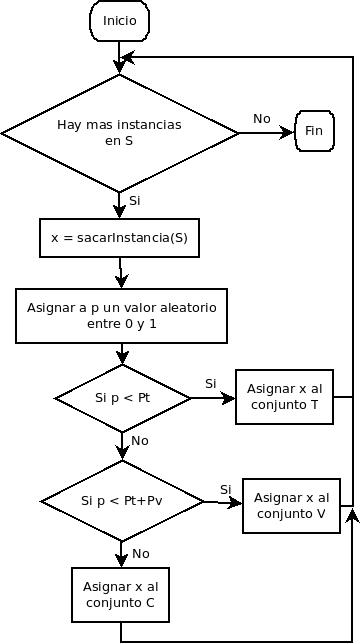
\includegraphics[width=7cm]{diagrams/setPartition.jpg}
\end{center}
\caption{Procedimiento para producir los conjuntos de entrenamiento y validación}
\label{fig:setPartition}
\end{figure}

\subsection{Mediciones}

Una vez entrenado el modelo de la distribución normal multivariable como se explicó en el capitulo \ref{chap:ml}, se llevaron a cabo las mediciones de precisión sobre las instancias del conjunto de validación, es decir, aquellas instancias que no fueron utilizadas en el proceso de entrenamiento. Para esto se utilizó el modelo entrenado y se observaron las predicciones realizadas por este modelo sobre este conjunto de validación. Dado que en el proceso de construcción de conjunto de validación cada componente fue etiquetado se conocía cual era la salida esperada para cada instancia con la que se probaba el modelo. En términos formales, el conjunto de entrenamiento $V$ se podría definir de la siguiente manera:

\[ V = \{\vec{x_i},r_i\}_{i=0}^N \]

Donde $N$ es la cantidad de elementos del conjunto de validación y $r_i$ es la salida esperada para el valor de entrada $\vec{x}_i$. Supongamos que la salida observada del modelo entrenado para el valor $\vec{x_i}$ es $y_i$, entonces se considera que el clasificador comete un error si $r_i \ne y_i$ y acierta si $r_i = y_i$. Considerando que cada acierto cuenta  una igualdad tenga por valor 1 si es verdadera y 0 si es falsa, entonces el valor medido se calcula de la siguiente forma:
\[ A = \frac{1}{N} \sum_{j=0}^{N}(r_i=y_i) \]
Se puede observar que el valor medido $A$ significa la cantidad de aciertos sobre el número total de intentos de predicción. Y por tanto mide el porcentaje de efectividad del clasificador para el problema de reconocimiento de caracteres.

\chapter{Diseño, implementación y pruebas del aplicativo}
\label{chap:ingSw}

 %\begin{Burocracy}
\section{Análisis}

La primera etapa en el desarrollo de software es la de levantamiento de requerimientos. Los requerimientos fueron tomados de los objetivos de desarrollo del proyecto (ver sección \ref{sect:objective}). Los objetivos exponen que se requiere desarrollar una aplicación para reconocimiento de dígitos que utilice para clasificar el modelo estadístico multivariable detallado en la sección \ref{sect:multivar} y para la extracción de características los momentos invariantes expuestos en la sección \ref{sect:invariants}.

Se determinó que es posible modelar la aplicación mediante dos casos de uso, ya que desde el punto de vista de los actores solo hay dos funciones que pueden desempeñar con la aplicación. El diagrama se muestra en la figura \ref{fig:useCase}. Un caso de uso, cuyo actor principal es un usuario administrador, se denomina ``entrenamiento del sistema de clasificación''. El otro caso de uso, que tiene como actor al usuario final, es el de ``reconocimiento de caracteres en el documento fotografiado''.

\begin{figure}[htb]
\begin{center}
\leavevmode
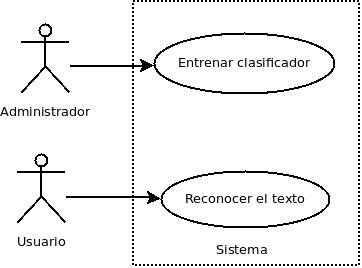
\includegraphics[width=7cm]{diagrams/casoUso.jpg}
\end{center}
\caption{Diagrama de casos de uso}
\label{fig:useCase}
\end{figure}

\subsection{Documentación de casos de uso}

La documentación de los casos de uso se encuentra en la tabla \ref{tb:uc1} y en la tabla \ref{tb:uc2}.

\begin{table}
\begin{center}
\begin{tabular}{|p{6cm}|p{6cm}|}
	\hline
	Caso de uso & Entrenamiento del sistema de clasificación\\
	\hline
	Actor: Usuario administrador & Referencia: 1 \\
	\hline
	Precondición: Sistema no entrenado. Imágenes de entrenamiento en un mismo directorio nombradas como se explica en la sección \ref{sect:testEnvironment} & 
	Postcondición: Sistema entrenado. \\
	\hline
	Sistema & Usuario \\
	\hline
	1. El usuario administrador indica en que directorio se encuentran las imágenes de entrenamiento. &
	2. El sistema construye un conjunto de entrenamiento como se explica en la sección \ref{sect:trainingSet} con todas las imágenes del directorio pasado por el usuario. \\
	\hline
	4. El usuario recibe un mensaje que indica que el procedimiento se realizó c\label{eq:hu}on éxito. &
	3. El sistema se entrena como se explica en el capítulo \ref{chap:ml} y guarda el modelo en disco. \\
	\hline
\end{tabular}
\end{center}
\caption{Caso de uso 1}	
\label{tb:uc1}
\end{table}

\begin{table}
\begin{center}
\begin{tabular}{|p{6cm}|p{6cm}|}
	\hline
	Caso de uso & Reconocimiento de caracteres en el documento fotografiado\\
	\hline
	Actor: Usuario final & Referencia: 2 \\
	\hline
	Precondición: Sistema entrenado & Postcondición: El usuario tiene el texto solicitado. \\
	\hline
	Sistema & Usuario \\
	\hline
	1. El usuario le envía al sistema una imagen del documento que desea leer. Las condiciones de captura de la imagen deben estar entre las especificadas en la sección \ref{sect:population}. &
	2. El sistema binariza la imagen, la segmenta y reconoce los caracteres segmentados en la imagen. \\
	\hline
	4. El usuario recibe el texto reconocido por el sistema &
	3. El sistema envía al usuario el texto reconocido de la imagen enviada. \\
	\hline
\end{tabular}
\end{center}
\caption{Caso de uso 2}	
\label{tb:uc2}
\end{table}

\section{Diseño}

El diseño del aplicativo se realizó con los diagramas de secuencia y clases pertenecientes al estándar UML. Los diagramas de secuencia se pueden apreciar en las figuras \ref{fig:sequence1} y \ref{fig:sequence2}.

\begin{sidewaysfigure}
\begin{center}
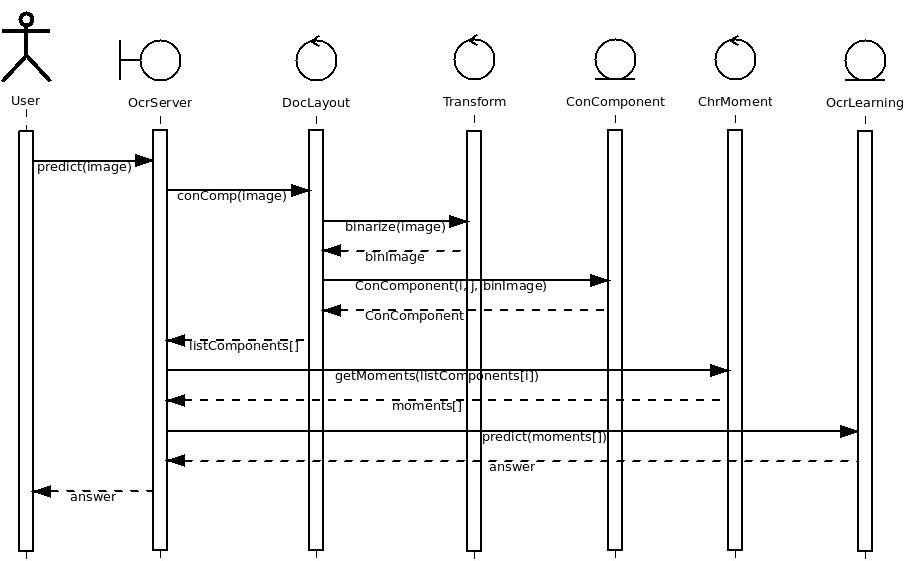
\includegraphics[width=20cm]{diagrams/sequence1.jpeg}
\end{center}
\caption{Diagrama de secuencia del primer caso de uso}
\label{fig:sequence1}
\end{sidewaysfigure}

\begin{sidewaysfigure}
\begin{center}
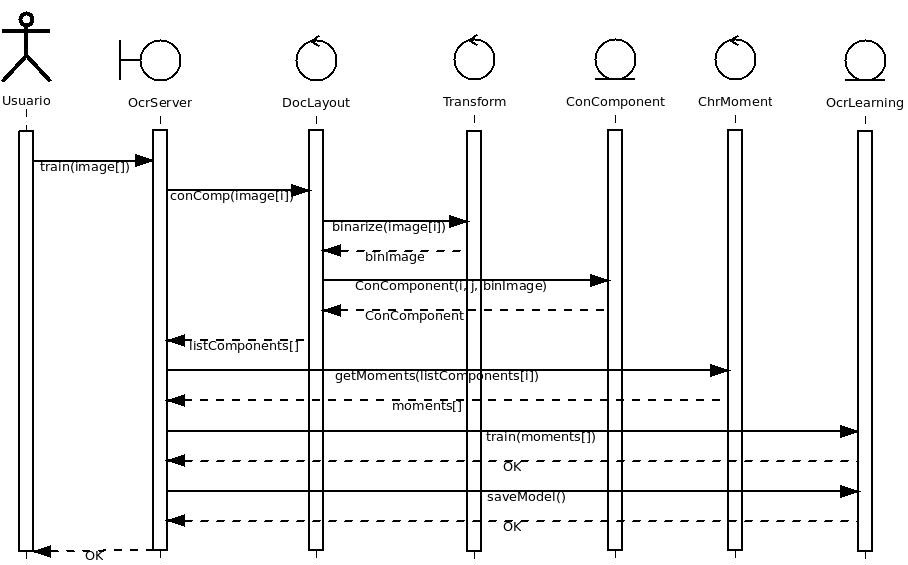
\includegraphics[width=20cm]{diagrams/sequence2.jpeg}
\end{center}
\caption{Diagrama de secuencia del segundo caso de uso}
\label{fig:sequence2}
\end{sidewaysfigure}

\begin{sidewaysfigure}
\begin{center}
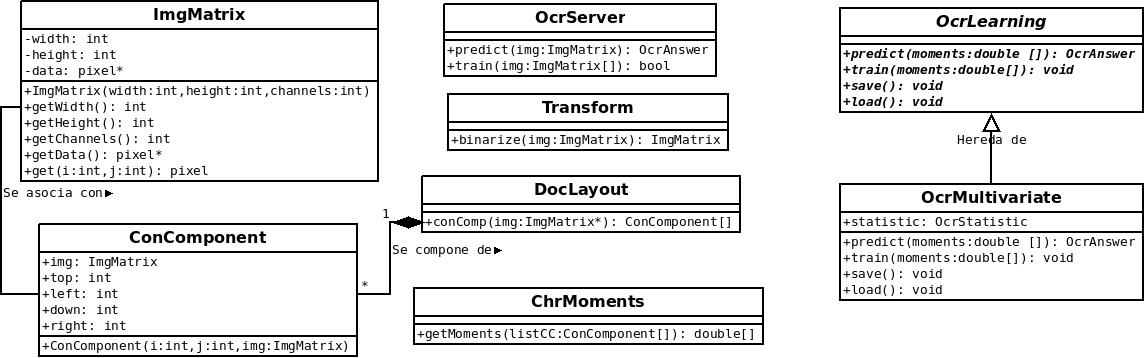
\includegraphics[width=20cm]{diagrams/clases.jpg}
\end{center}
\caption{Diagrama de clases}
\label{fig:classes}
\end{sidewaysfigure}

En el diagrama de clases (Fig. \ref{fig:classes}) se encuentran las clases con las que se pueden llevar a cabo los casos de uso con sus respectivos métodos públicos. La clase {\it ImgMatrix} es responsable de la representación de la imagen en el computador como una matriz. La clase {\it ConComponent} representa los componentes conectados de la imagen binarizada, hay un componente conectado por cada caracter de la imagen. La clase {\it OcrServer}, es la encargada de recibir las peticiones IP y coordinar las otras clases para dar respuesta a la petición. La clase {\it Transform} es la responsable de hacer la binarización de las imágenes con el algoritmo de Sauvola. La clase {\it DocLayout} es la responsable de dividir la imagen en los componentes conectados. La clase {\it ChrMoments} es responsable de calcular los momentos invariantes de Hu y Flusser para los componentes conectados, entregando un vector de características. Los momentos de Flusser implementados son tanto los momentos estándares, como los de momentos para objetos simétricos a N-rotaciones (Ver capítulo \ref{chap:features}), que se agregaron en el curso de la investigación.

La clase {\it OcrLearning} es una clase genérica que encapsula los métodos que debe tener un método de aprendizaje para la clasificación de caracteres. Se tomo la decisión de crear una clase padre porque en un futuro se pueden intentar métodos de aprendizaje distintos como redes neuronales, y el tener esta clase facilitaría la migración, ya que en este caso solo sería necesario crear otra clase que herede de {\it OcrLearning} con un método de aprendizaje nuevo. La clase {\it OcrMultivariate} es la que contiene la implementación de {\it OcrLearning} para el método específico de clasificación estadística, en la que se utiliza la distribución normal multivariable y el teorema de Bayes. Además de los métodos de entrenamiento y clasificación de los que se habló en el capítulo \ref{chap:ml}, se agregaron métodos de guardado y carga. La idea de estos dos métodos es que no sea necesario entrenar el método cada vez que se carga el programa, en cambio se puede guardar el modelo entrenado en un archivo en el disco y luego utilizarlo cada vez que se cargue el aplicativo.

\section{Pruebas}

En esta sección se explican las pruebas que se hicieron al software para determinar si los algoritmos fueron implementados correctamente. El objetivo de esta sección no es precisar si el resultado de los algoritmos es satisfactorio o no, ya que esto se explica en los capítulos \ref{chap:ml}, \ref{chap:features} y \ref{chap:results}.

Usualmente las pruebas se hacen creando un conjunto de casos de prueba para los que se conoce la salida esperada. En estos casos el proceso de pruebas consiste en alimentar al software con los casos de prueba y observar si la salida coincide con la salida esperada. Si la salida obtenida no coincide con la salida esperada, entonces se considera que el software tiene un error y se procede a depurarlo y corregirlo. Este proceso no garantiza un software libre de errores, pero si permite hallar muchos errores comunes y por tanto producir software de mejor calidad. Es de notar que los algoritmos de clasificación y de extracción de características implementados (descritos en los capítulos \ref{chap:ml} y \ref{chap:features}), son de una naturaleza matemática y, por tanto, no es fácil aplicarle este tipo de pruebas. Esto es debido a que muchas veces no es posible determinar cuál debería ser la salida esperada, pues para hacerlo se tendrían que realizar una gran cantidad de operaciones y solo un computador podría realizarlas en un tiempo razonable. 

\subsection{Etapas de preprocesamiento}

Para el cambio de color a escala de grises se compararon los resultados de la función implementada, y de una función de la librería OpenCV que realizaba el mismo procedimiento. La binarización se implementó en la clase {\it Transform}, como se explicó en la sección \ref{sect:binarization}. Dado que el mismo método esta implementado en {\it Ocropus} \footnote{Ocropus es un software de OCR libre desarrollado por Google, esta licenciado bajo Apache Licence 2.0}, la forma en la que se probó la implementación fue la siguiente:

	\begin{enumerate}
	\item Se tomaron 5 imágenes de documentos.
	\item Para cada foto, se binarizaron utilizando {\it Ocropus} y la clase {\it Transform}.
	\item Se compararon las imágenes resultado de la binarización con ambos métodos para comprobar que fueran iguales.
	\end{enumerate}

\subsection{Extracción de características}

Esta etapa fue un reto en cuanto a las pruebas de software, dado que, por el gran número de ecuaciones, era fácil cometer errores y difícil encontrarlos. En el capítulo \ref{chap:features} se explica que en la extracción de características la entrada es una imagen y la salida es un vector numérico calculado sobre la imagen. En el caso especial de los momentos invariantes, que fueron las características escogidas e implementadas, el vector se calcula con una integral sobre la imagen, que se convierte en una sumatoria de los píxeles de la imagen.

Dada la gran cantidad de píxeles, para un ser humano es difícil saber cuál es el vector numérico de salida a partir de una imagen de entrada. Además de esto, las fórmulas son bastante extensas (ver ecuaciones \ref{eq:huMom}) y por tanto es fácil cometer algún error en su implementación. Por estas razones, las pruebas se hicieron de la siguiente manera:

	\begin{enumerate}

	\item Los momentos de Hu fueron implementados por 2 personas diferentes, es decir, se realizó una doble implementación de las funciones que los calculaban. Se consideró que este método de implementación minimiza la posibilidad de que los errores no sean detectados, por cuanto la probabilidad de que dos personas cometan exactamente el mismo error es muy baja.
	
	\item Los momentos de Flusser fueron probados de la siguiente manera: para cada componente del conjunto de entrenamiento se calcularon los momentos de Flusser y de Hu y posteriormente se comprobaba si los de Flusser estaban bien revisando las equivalencias matemáticas que deben existir entre ambos vectores de características. %De esta forma los momentos de Flusser fueron implementados en realidad tres veces.
	
	\item Dado que los momentos de Hu son un subconjunto de los de Flusser, no era posible probar todos los momentos de Flusser con los Hu. Para probar los momentos de Flusser restantes se utilizo el hecho de que estos momentos son invariantes a la rotación, así que la última prueba consistió en rotar todas las imágenes 90$^\circ$, 180$^\circ$ y 270$^\circ$, y verificar que los valores fueran similares.
	
	\end{enumerate}

Gracias al punto 1, se detectó un error en un signo de los momentos de Hu en una de las implementaciones, y se corrigió el problema. El resto de los momentos coincidieron en ambas implementaciones. Al hacer las comprobaciones del punto 2, no se detectó ningún error, aunque como se explicó anteriormente, esto prueba solo parte de los momentos, no todos. Con el punto 3 de las comprobaciones, se detectó un cambio de signo al rotar la imagen en una de las variables del vector de características. Al revisar el código se detectó que el problema era causado por un error de digitación en el exponente de la formula, así que se corrigió.

\subsection{Distribución normal multivariable y clasificación}

Para calcular el determinante de las matrices de covarianza y la distancia Mahalanobis se utilizaron las funciones de la librería OpenCV {\it cvCalcCovarMatrix}, {\it cvMahalanobis} y {\it cvInvert} para realizar el cálculo de la matriz de covarianza, la distancia Mahalanobis y de la inversa de una matriz respectivamente. Estas funciones han sido probadas extensamente por la comunidad de desarrolladores de OpenCV desde el lanzamiento de esta librería en el año 2000, y cabe anotar que son estas funciones en las que se pueden cometer errores más fácilmente.

Para probar el resto de la lógica referente a los modelos estadísticos y la clasificación, se comprobaron las equivalencias que debían existir entre las etapas de los diferentes métodos implementados. Por ejemplo se comprobó que el resultado del método de distancia de Mahalanobis usando una matriz de covarianza diferente para cada instancia fuera equivalente al resultado del método de distribución normal multivariable con matriz de covarianza semi-compartida.

\chapter{Análisis de los datos, conclusiones y resultados}
\label{chap:results}

A lo largo de este documento, se ha expuesto el diseño general de un sistema de reconocimiento óptico de caracteres y se han mostrado técnicas y algoritmos existentes para cada una de las etapas. Además de cada etapa se seleccionó algún algoritmo o grupo de algoritmos que por sus características teóricas resultaban mejores para el problema OCR, y se explicaron las razones por las cuales se habían escogido los algoritmos que se implementaron y se mostraron los resultados de estos algoritmos sobre el proyecto.

\section{Resultados de la investigación}

Como ya se ha expuesto a lo largo del documento, el sistema de reconocimiento óptico de caracteres al igual que otros sistemas de visión por computador, se divide en tres etapas principales: el preprocesamiento (binarización, filtrado y segmentación de la imagen), la extracción de características (entrega un vector de números que representa las características deseadas de la imagen) y el reconocimiento (clasificación del vector de características usando aprendizaje de máquinas).

\subsection{Etapas de preprocesamiento}

Para la etapa de preprocesamiento se utilizaron 3 algoritmos para cada una de sus sub-etapas. En la sub-etapa de binarización se utilizó el algoritmo de Sauvola con la mejora en tiempo de Breuel, los resultados de la binarización se muestran en la sección \ref{sect:binarization}. En la implementación del algoritmo de binarización se cambió la forma en la que se referenciaba la memoria para lograr aún mejores tiempos de respuesta, con esta mejora se disminuyó el tiempo a $\frac{1}{5}$ del tiempo de la implementación original de Breuel para imágenes de 4 mega píxeles. %, los resultados detallados se muestran en la tabla \ref{tb:sauvolaFast}.
La sub-etapa de segmentación, que divide la imagen en los componentes de interés, se implementó con un algoritmo de Flood-fill como se explica en la sección \ref{sect:conComponents}. Para la sub-etapa de filtrado se aplicaron condiciones sobre el tamaño de los componentes obtenidos en la sub-etapa de segmentación, ya que otros métodos comunes como filtros Gaussianos causaban daños a la imagen que no permitían luego una correcta segmentación.

\subsection{Etapa de extracción de características}

En la etapa de extracción de características, el reto era conseguir buenas características que fueran invariantes a la rotación. Era necesario tener características invariantes a la rotación ya que es difícil que una persona invidente pueda tomar una imagen siempre con el mismo ángulo de rotación. En el capítulo \ref{chap:features} se exploraron diferentes conjuntos de características que podían resolver el problema con diferentes enfoques y se seleccionaron 3 explicando por qué las otras características no eran buenas para el reconocimiento de caracteres bajo las condiciones deseadas. 

Las características seleccionadas fueron los momentos invariantes de Hu, Flusser y los de Flusser para simetría a la rotación. El funcionamiento de cada uno de estos conjuntos de características y las razones matemáticas por las que podían dar un buen resultado para el problema del reconocimiento óptico de caracteres se exponen en el capítulo \ref{chap:features}.

Los resultados de estos 3 conjuntos de características fueron en general buenos. Para el mejor método de clasificación el conjunto de características con el resultado más bajo fue el de Hu con una precisión del 98.18\% para el reconocimiento de dígitos (Vea la tabla \ref{tb:exp4_2}). Teniendo en cuenta que la cantidad de símbolos en este experimento son 10 (Los dígitos del 0 al 9), un método de elección aleatoria tendría una respuesta correcta en un 10\% de los casos, el rendimiento de los momentos invariantes es en general muy bueno.

De estos 3 conjuntos de características, para el mejor método de clasificación probado en los experimentos, el conjunto de características con mejor resultado fue el de Flusser para la simetría a la rotación con un porcentaje de precisión del 100\%, el siguiente fue el conjunto de Flusser con un porcentaje de precisión del 98.77\% y el siguiente fue el conjunto de Hu con un porcentaje de precisión del 98.18\%. Para la clasificación de dígitos realmente no fue mucha la diferencia entre los momentos de Flusser y lo de Hu. Sin embargo los momentos de Flusser para objetos simétricos a la rotación obtuvieron un porcentaje mayor debido a que dígitos como el 0 y el 8 tienen un cierto grado de simetría que causa confusión en los dos primeros conjuntos de características. 

Cabe anotar que un resultado de 100\% no quiere decir que el software nunca se vaya a equivocar, lo que este porcentaje indica es que en el conjunto de instancias de validación (que contiene 7461 instancias) el software no cometió ningún error. Sin embargo se pueden obtener conclusiones estadísticas, supongamos que hay una población infinita de posibles instancias de los dígitos, y tomamos una muestra de $n$ instancias. De cada instancia se dice que se clasificó correctamente con una probabilidad $p$ y que se cometió un error con una probabilidad $(1-p)$, esto corresponde perfectamente a una distribución de probabilidad binomial. Deseamos calcular cual es la probabilidad $a$ de que $p>p_i$, esto es:

\begin{align}
	p_i^n &= (1-a) \notag \\
	a &= 1-p_i^n \label{eq:binomProb}
\end{align}

Dado que en el experimento realizado $n=7461$, la probabilidad de que la precisión del sistema para el reconocimiento de números en las condiciones especificadas sea mayor a 99,9\% se calcula usando la ecuación \ref{eq:binomProb} y es del 99,94\%.

\subsection{Etapa de clasificación}

Para la etapa de clasificación se exploraron distintos algoritmos que se explican brevemente en el capítulo \ref{chap:ml}. Los algoritmos de bajo poder clasificatorio, como los árboles binarios de decisión, no son buenos para el problema OCR. para el problema OCR usualmente se usan los algoritmos más potentes como las redes neuronales, que no exigen separabilidad lineal. Sin embargo se tomo la decisión de no utilizar redes neuronales porque son difíciles de depurar, entonces en caso que el resultado del sistema no sea bueno, no se puede detectar fácilmente que parte del sistema no funciona correctamente. Por otro lado, las características utilizadas en este diseño de sistema son buenas y teóricamente generaban vectores separables linealmente para cada clase.

Por esta razón se consideró utilizar el método estadístico de distribución normal multivariable explicado en la sección \ref{sect:multivar}, y dado que se sabía que las características podían entregar vectores cercanos a cero, se consideró una variación de este método, propuesta por los autores, en la que la matriz de covarianza se compartía en el coeficiente pero no en el exponente, a la que le fue dada el nombre de distribución multivariable con matriz de covarianza semi-compartida. Los resultados para cada uno de los métodos se pueden apreciar en las tablas \ref{tb:exp1_1}, \ref{tb:exp1_2}, \ref{tb:exp2_1} y \ref{tb:exp2_2}.

La experiencia mostró que el método de matriz de covarianza semi-compartida tuvo mejor resultado en todos los experimentos. El método modificado es mejor para las características escogidas porque estas tienen una varianza pequeña, por lo que el determinante de la matriz de covarianza tiende a cero y causa gran inestabilidad al estar en el denominador (ver ecuaciones \ref{eq:multivariate} y \ref{eq:semishared}).

\section{Resultados finales con los números}

En esta sección se presentan los resultados finales obtenidos por el sistema en el reconocimiento de dígitos ya explicados a lo largo de este documento. Las tablas que muestran los resultados del reconocimiento de los dígitos numéricos muestran la tasa de reconocimiento para cada una de las clases. La comunidad científica que trabaja en el tema de aprendizaje de máquinas propone que los errores y aciertos del sistema de reconocimiento se deben dar en términos de verdaderos positivos (TP), verdaderos negativos (TN), falsos positivos (FP) y falsos negativos (FN). Para explicar en qué consisten estos conceptos veamos el ejemplo del símbolo '8' en la tabla \ref{tb:numHuIndep}. La tabla indica que el ocho tiene 341 verdaderos positivos, 3077 verdaderos negativos, 250 falsos positivos y 22 falsos negativos. Esto quiere decir que 341 instancias que se debían reconocer como ocho efectivamente se reconocieron como ochos; 3077 instancias que no se debían reconocer como ocho, efectivamente no se reconocieron como ochos; 250 instancias que no se debían reconocer como ochos, se reconocieron como ochos; y 22 instancias que se debían reconocer como ochos no se reconocieron como ochos. Los resultados obtenidos en estas tablas son distintos a los resultados presentados en el capitulo de construcción del sistema debido a que, para esta publicación final de resultados, se generaron nuevamente los conjuntos de validación y entrenamiento. De esta manera se pudo demostrar que el algoritmo tiene capacidad de generalización. Los resultados confirman que el sistema construido, ademas de poder generalizar, es bastante preciso, pues obtuvo nuevamente un 100% de efectividad en el  experimento de matriz de covarianza semi-compartida con momentos de Fluzzer N-fold.

\begin{table}
\centering
\begin{tabular}{|c|c|c|c|c|c|}
	\hline
	Símbolo & TP & TN & FP & FN & Precisión \\ 
	\hline
	0 & 366 & 3273 & 51 & 0 & 100.000000\% \\ 
	1 & 370 & 3320 & 0 & 0 & 100.000000\% \\ 
	2 & 255 & 3306 & 0 & 129 & 66.406250\% \\ 
	3 & 342 & 3348 & 0 & 0 & 100.000000\% \\ 
	4 & 384 & 3306 & 0 & 0 & 100.000000\% \\ 
	5 & 110 & 3324 & 0 & 256 & 30.054646\% \\ 
	6 & 338 & 3337 & 0 & 15 & 95.750710\% \\ 
	7 & 367 & 3323 & 0 & 0 & 100.000000\% \\ 
	8 & 341 & 3077 & 250 & 22 & 93.939392\% \\ 
	9 & 387 & 3166 & 129 & 8 & 97.974686\% \\ 
	\hline
	Total & 3260 & N/A & \multicolumn{2}{|c|}{430} & 88.346878\% \\
	\hline
\end{tabular}
\caption{Resultados con las características de Hu (matriz de covarianza independiente)}
\label{tb:numHuIndep}
\end{table}

\begin{table}
\centering
\begin{tabular}{|c|c|c|c|c|c|}
	\hline
	Símbolo & TP & TN & FP & FN & Precisión \\ 
	\hline
	0 & 366 & 3247 & 77 & 0 & 100.000000\% \\ 
	1 & 370 & 3320 & 0 & 0 & 100.000000\% \\ 
	2 & 304 & 3306 & 0 & 80 & 79.166664\% \\ 
	3 & 342 & 3348 & 0 & 0 & 100.000000\% \\ 
	4 & 375 & 3306 & 0 & 9 & 97.656250\% \\ 
	5 & 152 & 3323 & 1 & 214 & 41.530056\% \\ 
	6 & 334 & 3337 & 0 & 19 & 94.617561\% \\ 
	7 & 367 & 3323 & 0 & 0 & 100.000000\% \\ 
	8 & 358 & 3145 & 182 & 5 & 98.622589\% \\ 
	9 & 383 & 3216 & 79 & 12 & 96.962029\% \\ 
	\hline
	Total & 3351 & N/A & \multicolumn{2}{|c|}{339} & 90.813011\% \\
	\hline
\end{tabular}
\caption{Resultados con las características de Flusser (matriz de covarianza independiente)}
\label{tb:numFlIndep}
\end{table}

\begin{table}
\centering
\begin{tabular}{|c|c|c|c|c|c|}
	\hline
	Símbolo & TP & TN & FP & FN & Precisión \\ 
	\hline
	0 & 366 & 3324 & 0 & 0 & 100.000000\% \\ 
	1 & 370 & 3320 & 0 & 0 & 100.000000\% \\ 
	2 & 181 & 3306 & 0 & 203 & 47.135418\% \\ 
	3 & 340 & 3145 & 203 & 2 & 99.415207\% \\ 
	4 & 384 & 3306 & 0 & 0 & 100.000000\% \\ 
	5 & 366 & 3324 & 0 & 0 & 100.000000\% \\ 
	6 & 353 & 3337 & 0 & 0 & 100.000000\% \\ 
	7 & 367 & 3323 & 0 & 0 & 100.000000\% \\ 
	8 & 363 & 3325 & 2 & 0 & 100.000000\% \\ 
	9 & 395 & 3295 & 0 & 0 & 100.000000\% \\ 
	\hline
	Total & 3485 & N/A & \multicolumn{2}{|c|}{205} & 94.444443\% \\
	\hline
\end{tabular}
\caption{Resultados con las características de Flusser N-fold (matriz de covarianza independiente)}
\label{tb:numRotIndep}
\end{table}

\begin{table}
\centering
\begin{tabular}{|c|c|c|c|c|c|}
	\hline
	Símbolo & TP & TN & FP & FN & Precisión \\ 
	\hline
	0 & 362 & 3324 & 0 & 4 & 98.907104\% \\ 
	1 & 370 & 3320 & 0 & 0 & 100.000000\% \\ 
	2 & 384 & 3262 & 44 & 0 & 100.000000\% \\ 
	3 & 342 & 3348 & 0 & 0 & 100.000000\% \\ 
	4 & 384 & 3306 & 0 & 0 & 100.000000\% \\ 
	5 & 341 & 3283 & 41 & 25 & 93.169395\% \\ 
	6 & 351 & 3335 & 2 & 2 & 99.433426\% \\ 
	7 & 367 & 3323 & 0 & 0 & 100.000000\% \\ 
	8 & 311 & 3327 & 0 & 52 & 85.674934\% \\ 
	9 & 390 & 3294 & 1 & 5 & 98.734177\% \\ 
	\hline
	Total & 3602 & N/A & \multicolumn{2}{|c|}{88} & 97.615173\% \\
	\hline
\end{tabular}
\caption{Resultados con las características de Hu (matriz de covarianza semi-compartida)}
\label{tb:numHuShared}
\end{table}

\begin{table}
\centering
\begin{tabular}{|c|c|c|c|c|c|}
	\hline
	Símbolo & TP & TN & FP & FN & Precisión \\ 
	\hline
	0 & 361 & 3324 & 0 & 5 & 98.633881\% \\ 
	1 & 370 & 3320 & 0 & 0 & 100.000000\% \\ 
	2 & 384 & 3280 & 26 & 0 & 100.000000\% \\ 
	3 & 342 & 3348 & 0 & 0 & 100.000000\% \\ 
	4 & 384 & 3306 & 0 & 0 & 100.000000\% \\ 
	5 & 362 & 3302 & 22 & 4 & 98.907104\% \\ 
	6 & 352 & 3335 & 2 & 1 & 99.716713\% \\ 
	7 & 367 & 3323 & 0 & 0 & 100.000000\% \\ 
	8 & 338 & 3326 & 1 & 25 & 93.112946\% \\ 
	9 & 379 & 3295 & 0 & 16 & 95.949364\% \\ 
	\hline
	Total & 3639 & N/A & \multicolumn{2}{|c|}{51} & 98.617889\% \\
	\hline
\end{tabular}
\caption{Resultados con las características de Flusser (matriz de covarianza semi-compartida)}
\label{tb:numFlShared}
\end{table}

\begin{table}
\centering
\begin{tabular}{|c|c|c|c|c|c|}
	\hline
	Símbolo & TP & TN & FP & FN & Precisión \\ 
	\hline
	0 & 366 & 3324 & 0 & 0 & 100.000000\% \\ 
	1 & 370 & 3320 & 0 & 0 & 100.000000\% \\ 
	2 & 384 & 3306 & 0 & 0 & 100.000000\% \\ 
	3 & 342 & 3348 & 0 & 0 & 100.000000\% \\ 
	4 & 384 & 3306 & 0 & 0 & 100.000000\% \\ 
	5 & 366 & 3324 & 0 & 0 & 100.000000\% \\ 
	6 & 353 & 3337 & 0 & 0 & 100.000000\% \\ 
	7 & 367 & 3323 & 0 & 0 & 100.000000\% \\ 
	8 & 363 & 3327 & 0 & 0 & 100.000000\% \\ 
	9 & 395 & 3295 & 0 & 0 & 100.000000\% \\ 
	\hline
	Total & 3690 & N/A & \multicolumn{2}{|c|}{0} & 100.000000\% \\
	\hline
\end{tabular}
\caption{Resultados con las características de Flusser N-fold (matriz de covarianza semi-compartida)}
\label{tb:numRotShared}
\end{table}

\section{Resultados al ingresar el alfabeto}

Aunque los objetivos iníciales consistían en trabajar solamente con dígitos numéricos, se tomo la decisión de ingresar los caracteres del alfabeto (únicamente de letras mayúsculas) debido al buen resultado obtenido con los caracteres numéricos. Los resultados del reconocimiento de caracteres para el método de reconocimiento de distribución normal multivariable con matriz semi-compartida se presenta en las tablas \ref{tb:alphaHuShared}, \ref{tb:alphaFlShared} y \ref{tb:alphaRotShared} para las características invariantes de Hu, Flusser y Flusser para simetría a la rotación respectivamente. Los resultados del reconocimiento de caracteres para el método de reconocimiento de distribución normal multivariable con matriz independiente se presenta en las tablas \ref{tb:alphaHuIndep}, \ref{tb:alphaFlIndep} y \ref{tb:alphaRotIndep} para las características invariantes de Hu, Flusser y Flusser para simetría a la rotación respectivamente. La efectividad relativa entre los dos metodos se mantuvo.

\begin{table}
\centering
\begin{tabular}{|c|c|c|c|c|c|}
	\hline
	Símbolo & TP & TN & FP & FN & Precisión \\ 
	\hline
	0 & 853 & 26099 & 7 & 106 & 88.946823\% \\ 
	1 & 956 & 26109 & 0 & 0 & 100.000000\% \\ 
	2 & 981 & 26037 & 45 & 2 & 99.796539\% \\ 
	3 & 967 & 26098 & 0 & 0 & 100.000000\% \\ 
	4 & 1015 & 26050 & 0 & 0 & 100.000000\% \\ 
	5 & 882 & 25931 & 129 & 123 & 87.761192\% \\ 
	6 & 968 & 26068 & 0 & 29 & 97.091270\% \\ 
	7 & 931 & 26134 & 0 & 0 & 100.000000\% \\ 
	8 & 852 & 26064 & 0 & 149 & 85.114883\% \\ 
	9 & 971 & 26049 & 0 & 45 & 95.570869\% \\ 
	A & 496 & 26569 & 0 & 0 & 100.000000\% \\ 
	B & 618 & 26318 & 0 & 129 & 82.730927\% \\ 
	C & 510 & 26555 & 0 & 0 & 100.000000\% \\ 
	D & 632 & 26378 & 0 & 55 & 91.994179\% \\ 
	E & 786 & 26279 & 0 & 0 & 100.000000\% \\ 
	F & 937 & 26128 & 0 & 0 & 100.000000\% \\ 
	G & 636 & 26291 & 5 & 133 & 82.704811\% \\ 
	H & 741 & 26108 & 126 & 90 & 89.169678\% \\ 
	I & 1298 & 25756 & 0 & 11 & 99.159660\% \\ 
	J & 886 & 26176 & 0 & 3 & 99.662544\% \\ 
	K & 688 & 26370 & 5 & 2 & 99.710144\% \\ 
	L & 903 & 26156 & 6 & 0 & 100.000000\% \\ 
	M & 31 & 26725 & 0 & 309 & 9.117647\% \\ 
	N & 474 & 26440 & 1 & 150 & 75.961540\% \\ 
	O & 232 & 26711 & 0 & 122 & 65.536720\% \\ 
	P & 786 & 26278 & 0 & 1 & 99.872932\% \\ 
	Q & 411 & 26593 & 52 & 9 & 97.857140\% \\ 
	R & 578 & 26484 & 0 & 3 & 99.483650\% \\ 
	S & 406 & 26313 & 8 & 338 & 54.569893\% \\ 
	T & 636 & 26429 & 0 & 0 & 100.000000\% \\ 
	U & 707 & 26358 & 0 & 0 & 100.000000\% \\ 
	V & 518 & 26543 & 2 & 2 & 99.615387\% \\ 
	W & 2 & 26989 & 5 & 69 & 2.816901\% \\ 
	X & 566 & 24931 & 1560 & 8 & 98.606270\% \\ 
	Y & 614 & 26450 & 0 & 1 & 99.837395\% \\ 
	Z & 645 & 26356 & 1 & 63 & 91.101692\% \\ 
	\hline
	Total & 25113 & N/A & \multicolumn{2}{|c|}{1952} & 92.7877\% \\
	\hline
\end{tabular}
\caption{Resultados con el alfabeto utilizando momentos de Hu (matriz semi-compartida)}
\label{tb:alphaHuShared}
\end{table}

\begin{table}
\centering
\begin{tabular}{|c|c|c|c|c|c|}
	\hline
	Símbolo & TP & TN & FP & FN & Precisión \\ 
	\hline
	0 & 944 & 26099 & 7 & 15 & 98.435867\% \\ 
	1 & 956 & 26106 & 3 & 0 & 100.000000\% \\ 
	2 & 982 & 25883 & 199 & 1 & 99.898270\% \\ 
	3 & 967 & 26098 & 0 & 0 & 100.000000\% \\ 
	4 & 1014 & 26050 & 0 & 1 & 99.901482\% \\ 
	5 & 996 & 25572 & 488 & 9 & 99.104477\% \\ 
	6 & 991 & 26068 & 0 & 6 & 99.398193\% \\ 
	7 & 931 & 26134 & 0 & 0 & 100.000000\% \\ 
	8 & 932 & 26016 & 48 & 69 & 93.106895\% \\ 
	9 & 987 & 26049 & 0 & 29 & 97.145668\% \\ 
	A & 496 & 26569 & 0 & 0 & 100.000000\% \\ 
	B & 661 & 26315 & 3 & 86 & 88.487282\% \\ 
	C & 510 & 26555 & 0 & 0 & 100.000000\% \\ 
	D & 614 & 26378 & 0 & 73 & 89.374092\% \\ 
	E & 786 & 26279 & 0 & 0 & 100.000000\% \\ 
	F & 936 & 26128 & 0 & 1 & 99.893280\% \\ 
	G & 769 & 26227 & 69 & 0 & 100.000000\% \\ 
	H & 765 & 26210 & 24 & 66 & 92.057762\% \\ 
	I & 1302 & 25717 & 39 & 7 & 99.465240\% \\ 
	J & 889 & 26176 & 0 & 0 & 100.000000\% \\ 
	K & 688 & 26374 & 1 & 2 & 99.710144\% \\ 
	L & 903 & 26157 & 5 & 0 & 100.000000\% \\ 
	M & 320 & 26725 & 0 & 20 & 94.117645\% \\ 
	N & 234 & 26441 & 0 & 390 & 37.500000\% \\ 
	O & 347 & 26711 & 0 & 7 & 98.022598\% \\ 
	P & 786 & 26278 & 0 & 1 & 99.872932\% \\ 
	Q & 419 & 26633 & 12 & 1 & 99.761902\% \\ 
	R & 581 & 26484 & 0 & 0 & 100.000000\% \\ 
	S & 705 & 26317 & 4 & 39 & 94.758064\% \\ 
	T & 636 & 26424 & 5 & 0 & 100.000000\% \\ 
	U & 707 & 26358 & 0 & 0 & 100.000000\% \\ 
	V & 518 & 26541 & 4 & 2 & 99.615387\% \\ 
	W & 16 & 26994 & 0 & 55 & 22.535212\% \\ 
	X & 562 & 26490 & 1 & 12 & 97.909409\% \\ 
	Y & 596 & 26449 & 1 & 19 & 96.910568\% \\ 
	Z & 697 & 26348 & 9 & 11 & 98.446327\% \\ 
	\hline
	Total & 26143 & N/A & \multicolumn{2}{|c|}{922} & 96.5934\% \\
	\hline
\end{tabular}
\caption{Resultados con el alfabeto utilizando momentos de Flusser (matriz semi-compartida)}
\label{tb:alphaFlShared}
\end{table}

\begin{table}
\centering
\begin{tabular}{|c|c|c|c|c|c|}
	\hline
	Símbolo & TP & TN & FP & FN & Precisión \\ 
	\hline
	0 & 959 & 26106 & 0 & 0 & 100.000000\% \\ 
	1 & 956 & 26109 & 0 & 0 & 100.000000\% \\ 
	2 & 982 & 26082 & 0 & 1 & 99.898270\% \\ 
	3 & 967 & 26098 & 0 & 0 & 100.000000\% \\ 
	4 & 1015 & 26050 & 0 & 0 & 100.000000\% \\ 
	5 & 1005 & 26060 & 0 & 0 & 100.000000\% \\ 
	6 & 997 & 26068 & 0 & 0 & 100.000000\% \\ 
	7 & 931 & 26134 & 0 & 0 & 100.000000\% \\ 
	8 & 1001 & 26064 & 0 & 0 & 100.000000\% \\ 
	9 & 1016 & 26049 & 0 & 0 & 100.000000\% \\ 
	A & 463 & 26569 & 0 & 33 & 93.346771\% \\ 
	B & 747 & 26318 & 0 & 0 & 100.000000\% \\ 
	C & 510 & 26555 & 0 & 0 & 100.000000\% \\ 
	D & 655 & 26378 & 0 & 32 & 95.342064\% \\ 
	E & 786 & 26262 & 17 & 0 & 100.000000\% \\ 
	F & 937 & 26128 & 0 & 0 & 100.000000\% \\ 
	G & 758 & 26296 & 0 & 11 & 98.569572\% \\ 
	H & 831 & 26179 & 55 & 0 & 100.000000\% \\ 
	I & 1309 & 25756 & 0 & 0 & 100.000000\% \\ 
	J & 889 & 26176 & 0 & 0 & 100.000000\% \\ 
	K & 688 & 26342 & 33 & 2 & 99.710144\% \\ 
	L & 903 & 26161 & 1 & 0 & 100.000000\% \\ 
	M & 319 & 26725 & 0 & 21 & 93.823532\% \\ 
	N & 579 & 26441 & 0 & 45 & 92.788460\% \\ 
	O & 354 & 26711 & 0 & 0 & 100.000000\% \\ 
	P & 786 & 26278 & 0 & 1 & 99.872932\% \\ 
	Q & 419 & 26602 & 43 & 1 & 99.761902\% \\ 
	R & 558 & 26484 & 0 & 23 & 96.041306\% \\ 
	S & 743 & 26321 & 0 & 1 & 99.865593\% \\ 
	T & 636 & 26429 & 0 & 0 & 100.000000\% \\ 
	U & 707 & 26358 & 0 & 0 & 100.000000\% \\ 
	V & 518 & 26512 & 33 & 2 & 99.615387\% \\ 
	W & 53 & 26989 & 5 & 18 & 74.647888\% \\ 
	X & 574 & 26484 & 7 & 0 & 100.000000\% \\ 
	Y & 612 & 26450 & 0 & 3 & 99.512192\% \\ 
	Z & 708 & 26357 & 0 & 0 & 100.000000\% \\ 
	\hline
	Total & 26871 & N/A & \multicolumn{2}{|c|}{194} & 99.283203\% \\
	\hline
\end{tabular}
\caption{Resultados con el alfabeto utilizando momentos de Flusser 2-Fold (matriz semi-compartida)}
\label{tb:alphaRotShared}
\end{table}

\begin{table}
\centering
\begin{tabular}{|c|c|c|c|c|c|}
	\hline
	Símbolo & TP & TN & FP & FN & Precisión \\ 
	\hline
	0 & 945 & 25963 & 143 & 14 & 98.540146\% \\ 
	1 & 956 & 26109 & 0 & 0 & 100.000000\% \\ 
	2 & 885 & 26081 & 1 & 98 & 90.030518\% \\ 
	3 & 967 & 26093 & 5 & 0 & 100.000000\% \\ 
	4 & 1013 & 26050 & 0 & 2 & 99.802956\% \\ 
	5 & 297 & 25976 & 84 & 708 & 29.552238\% \\ 
	6 & 934 & 26064 & 4 & 63 & 93.681046\% \\ 
	7 & 931 & 26134 & 0 & 0 & 100.000000\% \\ 
	8 & 948 & 25431 & 633 & 53 & 94.705292\% \\ 
	9 & 998 & 25892 & 157 & 18 & 98.228348\% \\ 
	A & 496 & 26569 & 0 & 0 & 100.000000\% \\ 
	B & 735 & 26121 & 197 & 12 & 98.393578\% \\ 
	C & 469 & 26555 & 0 & 41 & 91.960785\% \\ 
	D & 679 & 26259 & 119 & 8 & 98.835518\% \\ 
	E & 786 & 25631 & 648 & 0 & 100.000000\% \\ 
	F & 937 & 26128 & 0 & 0 & 100.000000\% \\ 
	G & 625 & 25832 & 464 & 144 & 81.274384\% \\ 
	H & 14 & 26234 & 0 & 817 & 1.684717\% \\ 
	I & 1308 & 25756 & 0 & 1 & 99.923607\% \\ 
	J & 889 & 26176 & 0 & 0 & 100.000000\% \\ 
	K & 76 & 26373 & 2 & 614 & 11.014493\% \\ 
	L & 903 & 26159 & 3 & 0 & 100.000000\% \\ 
	M & 337 & 26709 & 16 & 3 & 99.117645\% \\ 
	N & 624 & 25943 & 498 & 0 & 100.000000\% \\ 
	O & 127 & 26215 & 496 & 227 & 35.875706\% \\ 
	P & 786 & 26278 & 0 & 1 & 99.872932\% \\ 
	Q & 0 & 26645 & 0 & 420 & 0.000000\% \\ 
	R & 581 & 26484 & 0 & 0 & 100.000000\% \\ 
	S & 742 & 26027 & 294 & 2 & 99.731186\% \\ 
	T & 636 & 26429 & 0 & 0 & 100.000000\% \\ 
	U & 707 & 26358 & 0 & 0 & 100.000000\% \\ 
	V & 518 & 26543 & 2 & 2 & 99.615387\% \\ 
	W & 1 & 26991 & 3 & 70 & 1.408451\% \\ 
	X & 0 & 26490 & 1 & 574 & 0.000000\% \\ 
	Y & 614 & 26450 & 0 & 1 & 99.837395\% \\ 
	Z & 699 & 26225 & 132 & 9 & 98.728813\% \\ 
	\hline
	Total & 23163 & N/A & \multicolumn{2}{|c|}{3902} & 85.582855\% \\
	\hline
\end{tabular}
\caption{Resultados con el alfabeto utilizando momentos de Hu (matriz independiente)}
\label{tb:alphaHuIndep}
\end{table}

\begin{table}
\centering
\begin{tabular}{|c|c|c|c|c|c|}
	\hline
	Símbolo & TP & TN & FP & FN & Precisión \\ 
	\hline
	0 & 397 & 25042 & 1064 & 562 & 41.397289\% \\ 
	1 & 956 & 26105 & 4 & 0 & 100.000000\% \\ 
	2 & 881 & 25992 & 90 & 102 & 89.623604\% \\ 
	3 & 967 & 26098 & 0 & 0 & 100.000000\% \\ 
	4 & 975 & 26049 & 1 & 40 & 96.059113\% \\ 
	5 & 440 & 25594 & 466 & 565 & 43.781094\% \\ 
	6 & 912 & 26068 & 0 & 85 & 91.474426\% \\ 
	7 & 930 & 26134 & 0 & 1 & 99.892586\% \\ 
	8 & 712 & 25630 & 434 & 289 & 71.128868\% \\ 
	9 & 989 & 25994 & 55 & 27 & 97.342522\% \\ 
	A & 496 & 26567 & 2 & 0 & 100.000000\% \\ 
	B & 744 & 25863 & 455 & 3 & 99.598396\% \\ 
	C & 510 & 26555 & 0 & 0 & 100.000000\% \\ 
	D & 220 & 26149 & 229 & 467 & 32.023289\% \\ 
	E & 786 & 26279 & 0 & 0 & 100.000000\% \\ 
	F & 937 & 25800 & 328 & 0 & 100.000000\% \\ 
	G & 533 & 25936 & 360 & 236 & 69.310791\% \\ 
	H & 269 & 26234 & 0 & 562 & 32.370636\% \\ 
	I & 1225 & 25717 & 39 & 84 & 93.582886\% \\ 
	J & 889 & 26176 & 0 & 0 & 100.000000\% \\ 
	K & 360 & 26375 & 0 & 330 & 52.173912\% \\ 
	L & 903 & 26160 & 2 & 0 & 100.000000\% \\ 
	M & 338 & 26708 & 17 & 2 & 99.411766\% \\ 
	N & 624 & 25866 & 575 & 0 & 100.000000\% \\ 
	O & 354 & 26639 & 72 & 0 & 100.000000\% \\ 
	P & 786 & 26278 & 0 & 1 & 99.872932\% \\ 
	Q & 58 & 26645 & 0 & 362 & 13.809524\% \\ 
	R & 581 & 26483 & 1 & 0 & 100.000000\% \\ 
	S & 735 & 25735 & 586 & 9 & 98.790321\% \\ 
	T & 636 & 26428 & 1 & 0 & 100.000000\% \\ 
	U & 707 & 26358 & 0 & 0 & 100.000000\% \\ 
	V & 516 & 26544 & 1 & 4 & 99.230766\% \\ 
	W & 0 & 26994 & 0 & 71 & 0.000000\% \\ 
	X & 0 & 26491 & 0 & 574 & 0.000000\% \\ 
	Y & 152 & 26450 & 0 & 463 & 24.715446\% \\ 
	Z & 544 & 26136 & 221 & 164 & 76.836159\% \\ 
	\hline
	Total & 22062 & N/A & \multicolumn{2}{|c|}{5003} & 81.514870\% \\
	\hline
\end{tabular}
\caption{Resultados con el alfabeto utilizando momentos de flusser (matriz independiente)}
\label{tb:alphaFlIndep}
\end{table}

\begin{table}
\centering
\begin{tabular}{|c|c|c|c|c|c|}
	\hline
	Símbolo & TP & TN & FP & FN & Precisión \\ 
	\hline
	0 & 959 & 26106 & 0 & 0 & 100.000000\% \\ 
	1 & 956 & 26109 & 0 & 0 & 100.000000\% \\ 
	2 & 981 & 26082 & 0 & 2 & 99.796539\% \\ 
	3 & 959 & 26098 & 0 & 8 & 99.172699\% \\ 
	4 & 1015 & 26050 & 0 & 0 & 100.000000\% \\ 
	5 & 1005 & 26060 & 0 & 0 & 100.000000\% \\ 
	6 & 987 & 26062 & 6 & 10 & 98.996994\% \\ 
	7 & 931 & 26110 & 24 & 0 & 100.000000\% \\ 
	8 & 1001 & 26055 & 9 & 0 & 100.000000\% \\ 
	9 & 1014 & 26049 & 0 & 2 & 99.803146\% \\ 
	A & 496 & 25435 & 1134 & 0 & 100.000000\% \\ 
	B & 747 & 26259 & 59 & 0 & 100.000000\% \\ 
	C & 0 & 26555 & 0 & 510 & 0.000000\% \\ 
	D & 684 & 25924 & 454 & 3 & 99.563316\% \\ 
	E & 786 & 25556 & 723 & 0 & 100.000000\% \\ 
	F & 937 & 26128 & 0 & 0 & 100.000000\% \\ 
	G & 769 & 25874 & 422 & 0 & 100.000000\% \\ 
	H & 36 & 26234 & 0 & 795 & 4.332130\% \\ 
	I & 1309 & 25756 & 0 & 0 & 100.000000\% \\ 
	J & 889 & 26176 & 0 & 0 & 100.000000\% \\ 
	K & 0 & 26373 & 2 & 690 & 0.000000\% \\ 
	L & 877 & 26161 & 1 & 26 & 97.120712\% \\ 
	M & 338 & 26695 & 30 & 2 & 99.411766\% \\ 
	N & 624 & 25685 & 756 & 0 & 100.000000\% \\ 
	O & 354 & 26711 & 0 & 0 & 100.000000\% \\ 
	P & 786 & 26278 & 0 & 1 & 99.872932\% \\ 
	Q & 0 & 26645 & 0 & 420 & 0.000000\% \\ 
	R & 581 & 26479 & 5 & 0 & 100.000000\% \\ 
	S & 743 & 26319 & 2 & 1 & 99.865593\% \\ 
	T & 636 & 25811 & 618 & 0 & 100.000000\% \\ 
	U & 703 & 26358 & 0 & 4 & 99.434227\% \\ 
	V & 0 & 26544 & 1 & 520 & 0.000000\% \\ 
	W & 0 & 26990 & 4 & 71 & 0.000000\% \\ 
	X & 0 & 26487 & 4 & 574 & 0.000000\% \\ 
	Y & 0 & 26450 & 0 & 615 & 0.000000\% \\ 
	Z & 708 & 26357 & 0 & 0 & 100.000000\% \\ 
	\hline
	Total & 22811 & N/A & \multicolumn{2}{|c|}{4254} & 84.282288\% \\
	\hline
\end{tabular}
\caption{Resultados con el alfabeto utilizando momentos de flusser (matriz independiente)}
\label{tb:alphaRotIndep}
\end{table}

\section{Proyectos que se pueden derivar de esta investigación}

En esta investigación se desarrollo un sistema de reconocimiento óptico de caracteres para reconocer los dígitos del 0 al 9. Aunque se agregaron las letras mayúsculas, y los resultados fueron buenos, el sistema no está optimizado para utilizarlas. Así que el primer paso en un proyecto futuro sería desarrollar un sistema capaz de reconocer las letras del alfabeto latino, tanto mayúsculas como minúsculas, así como los signos de puntuación. Para hacerlo se tendrían que solucionar problemas como la separación de la letra minúscula i en dos componentes conectados, entre muchos otros que no fueron tratados en este proyecto.

El sistema desarrollado permite reconocer caracteres con tamaños entre 12 y 20 puntos, e imágenes con inclinaciones entre -30$^{\circ}$ y 30$^{\circ}$. No obstante, el problema se restringió a documentos con un mismo tipo de letra. En ejemplos de la vida real normalmente se encontrarían documentos con diversos tipos de letra, lo que aumentaría la complejidad del problema. En un proyecto futuro se podrían intentar varios enfoques para solucionar este problema. Una posibilidad es hacer un preprocesamiento para reconocer el tipo de letra de cada documento y posteriormente aplicarle un modelo ya entrenado al documento dependiendo del tipo de letra. Otra posibilidad es aplicar un método de aprendizaje no supervisado para separar en clusters todas las letras de la misma clase, sin importar su tipo de letra, y posteriormente realizar la clasificación con este nuevo modelo. El reto en estos casos sería no aumentar significativamente la complejidad computacional de la solución.

La etapa de reconocimiento de caracteres es muy importante, sin embargo, como fue explicado en el capitulo \ref{chap:intro}, es solo una de las etapas en el proceso de reconocimiento óptico de caracteres. Una etapa muy importante que no fue desarrollada en este proyecto es la de análisis del documento. Una gran ventaja que provee la solución estadística planteada en este proyecto es que, para cada componente conectado, se entrega un arreglo con las probabilidades de que el componente conectado pertenezca a cada clase. Esto podría ser especialmente útil para una etapa de post-procesamiento en el análisis del documento, en donde se podría utilizar un diccionario y modelos de Markov para determinar la probabilidad de que una secuencia de caracteres forme una palabra. De esta manera se podrían corregir fácilmente errores en los cuales se reconocieron erróneamente algunas letras de una palabra. Además de esto, para lograr un sistema de reconocimiento óptico de caracteres que pueda ser utilizado en la vida diaria por una persona invidente, es necesario realizar una etapa de análisis de documento que permita a distinguir palabras, líneas y frases.

El sistema planteado en este proyecto es solo uno de muchos aportes que la tecnología puede brindar a las personas invidentes. En un futuro no tan distante se podría desarrollar un sistema que reconozca no solo documentos, sino todo tipo de objetos en general. Este sistema podría darle al usuario, por medio de ayudas auditivas, un panorama general de todo lo que lo rodea. De esta manera se podría finalmente lograr que las personas invidentes no necesitaran de guías humanos ni caninos para desarrollar sus actividades cotidianas, lo que les permitiría ser más independientes y autónomos.

\begin{comment}
\chapter{GNU Free Documentation License}

0. PREÁMBULO

El propósito de esta Licencia es permitir que un manual, libro de texto, u otro documento escrito sea libre en el sentido de libertad: asegurar a todo el mundo la libertad efectiva de copiarlo y redistribuirlo, con o sin modificaciones, de manera comercial o no. En segundo término, esta Licencia proporciona al autor y al editor[2] una manera de obtener reconocimiento por su trabajo, sin que se le considere responsable de las modificaciones realizadas por otros.

Esta Licencia es de tipo copyleft, lo que significa que los trabajos derivados del documento deben a su vez ser libres en el mismo sentido. Complementa la Licencia Pública General de GNU, que es una licencia tipo copyleft diseñada para el software libre.

Hemos diseñado esta Licencia para usarla en manuales de software libre, ya que el software libre necesita documentación libre: un programa libre debe venir con manuales que ofrezcan la mismas libertades que el software. Pero esta licencia no se limita a manuales de software; puede usarse para cualquier texto, sin tener en cuenta su temática o si se publica como libro impreso o no. Recomendamos esta licencia principalmente para trabajos cuyo fin sea instructivo o de referencia.

1. APLICABILIDAD Y DEFINICIONES

Esta Licencia se aplica a cualquier manual u otro trabajo, en cualquier soporte, que contenga una nota del propietario de los derechos de autor que indique que puede ser distribuido bajo los términos de esta Licencia. Tal nota garantiza en cualquier lugar del mundo, sin pago de derechos y sin límite de tiempo, el uso de dicho trabajo según las condiciones aquí estipuladas. En adelante la palabra Documento se referirá a cualquiera de dichos manuales o trabajos. Cualquier persona es un licenciatario y será referido como Usted. Usted acepta la licencia si copia, modifica o distribuye el trabajo de cualquier modo que requiera permiso según la ley de propiedad intelectual.

Una Versión Modificada del Documento significa cualquier trabajo que contenga el Documento o una porción del mismo, ya sea una copia literal o con modificaciones y/o traducciones a otro idioma.

Una Sección Secundaria es un apéndice con título o una sección preliminar del Documento que trata exclusivamente de la relación entre los autores o editores y el tema general del Documento (o temas relacionados) pero que no contiene nada que entre directamente en dicho tema general (por ejemplo, si el Documento es en parte un texto de matemáticas, una Sección Secundaria puede no explicar nada de matemáticas). La relación puede ser una conexión histórica con el tema o temas relacionados, o una opinión legal, comercial, filosófica, ética o política acerca de ellos.

Las Secciones Invariantes son ciertas Secciones Secundarias cuyos títulos son designados como Secciones Invariantes en la nota que indica que el documento es liberado bajo esta Licencia. Si una sección no entra en la definición de Secundaria, no puede designarse como Invariante. El documento puede no tener Secciones Invariantes. Si el Documento no identifica las Secciones Invariantes, es que no las tiene.

Los Textos de Cubierta son ciertos pasajes cortos de texto que se listan como Textos de Cubierta Delantera o Textos de Cubierta Trasera en la nota que indica que el documento es liberado bajo esta Licencia. Un Texto de Cubierta Delantera puede tener como mucho 5 palabras, y uno de Cubierta Trasera puede tener hasta 25 palabras.

Una copia Transparente del Documento, significa una copia para lectura en máquina, representada en un formato cuya especificación está disponible al público en general, apto para que los contenidos puedan ser vistos y editados directamente con editores de texto genéricos o (para imágenes compuestas por puntos) con programas genéricos de manipulación de imágenes o (para dibujos) con algún editor de dibujos ampliamente disponible, y que sea adecuado como entrada para formateadores de texto o para su traducción automática a formatos adecuados para formateadores de texto. Una copia hecha en un formato definido como Transparente, pero cuyo marcaje o ausencia de él haya sido diseñado para impedir o dificultar modificaciones posteriores por parte de los lectores no es Transparente. Un formato de imagen no es Transparente si se usa para una cantidad de texto sustancial. Una copia que no es Transparente se denomina Opaca.

Como ejemplos de formatos adecuados para copias Transparentes están ASCII puro sin marcaje, formato de entrada de Texinfo, formato de entrada de LaTeX, SGML o XML usando una DTD disponible públicamente, y HTML, PostScript o PDF simples, que sigan los estándares y diseñados para que los modifiquen personas. Ejemplos de formatos de imagen transparentes son PNG, XCF y JPG. Los formatos Opacos incluyen formatos propietarios que pueden ser leídos y editados únicamente en procesadores de palabras propietarios, SGML o XML para los cuáles las DTD y/o herramientas de procesamiento no estén ampliamente disponibles, y HTML, PostScript o PDF generados por algunos procesadores de palabras sólo como salida.

La Portada significa, en un libro impreso, la página de título, más las páginas siguientes que sean necesarias para mantener, de manera legible, el material que esta Licencia requiere en la portada. Para trabajos en formatos que no tienen página de portada como tal, Portada significa el texto cercano a la aparición más prominente del título del trabajo, precediendo el comienzo del cuerpo del texto.

El Editor se refiere a cualquier persona o entidad que distribuya copias del Documento a el público.

Una sección Titulada XYZ significa una parte del Documento cuyo título es precisamente XYZ o contiene XYZ entre paréntesis, a continuación de texto que traduce XYZ a otro idioma (aquí XYZ se refiere a nombres de sección específicos mencionados más abajo, como Agradecimientos, Dedicatorias , Aprobaciones o Historia). Conservar el Título de tal sección cuando se modifica el Documento significa que permanece una sección Titulada XYZ según esta definición.[3]

El Documento puede incluir Limitaciones de Garantía cercanas a la nota donde se declara que al Documento se le aplica esta Licencia. Se considera que estas Limitaciones de Garantía están incluidas, por referencia, en la Licencia, pero sólo en cuanto a limitaciones de garantía: cualquier otra implicación que estas Limitaciones de Garantía puedan tener es nula y no tiene efecto en el significado de esta Licencia.

2. COPIA LITERAL

Usted puede copiar y distribuir el Documento en cualquier soporte, sea en forma comercial o no, siempre y cuando esta Licencia, las notas de copyright y la nota que indica que esta Licencia se aplica al Documento se reproduzcan en todas las copias y que usted no añada ninguna otra condición a las expuestas en esta Licencia. Usted no puede usar medidas técnicas para obstruir o controlar la lectura o copia posterior de las copias que usted haga o distribuya. Sin embargo, usted puede aceptar compensación a cambio de las copias. Si distribuye un número suficientemente grande de copias también deberá seguir las condiciones de la sección 3.

Usted también puede prestar copias, bajo las mismas condiciones establecidas anteriormente, y puede exhibir copias públicamente.

3. COPIADO EN CANTIDAD

Si publica copias impresas del Documento (o copias en soportes que tengan normalmente cubiertas impresas) que sobrepasen las 100, y la nota de licencia del Documento exige Textos de Cubierta, debe incluir las copias con cubiertas que lleven en forma clara y legible todos esos Textos de Cubierta: Textos de Cubierta Delantera en la cubierta delantera y Textos de Cubierta Trasera en la cubierta trasera. Ambas cubiertas deben identificarlo a Usted clara y legiblemente como editor de tales copias. La cubierta debe mostrar el título completo con todas las palabras igualmente prominentes y visibles. Además puede añadir otro material en las cubiertas. Las copias con cambios limitados a las cubiertas, siempre que conserven el título del Documento y satisfagan estas condiciones, pueden considerarse como copias literales.

Si los textos requeridos para la cubierta son muy voluminosos para que ajusten legiblemente, debe colocar los primeros (tantos como sea razonable colocar) en la verdadera cubierta y situar el resto en páginas adyacentes.

Si Usted publica o distribuye copias Opacas del Documento cuya cantidad exceda las 100, debe incluir una copia Transparente, que pueda ser leída por una máquina, con cada copia Opaca, o bien mostrar, en cada copia Opaca, una dirección de red donde cualquier usuario de la misma tenga acceso por medio de protocolos públicos y estandarizados a una copia Transparente del Documento completa, sin material adicional. Si usted hace uso de la última opción, deberá tomar las medidas necesarias, cuando comience la distribución de las copias Opacas en cantidad, para asegurar que esta copia Transparente permanecerá accesible en el sitio establecido por lo menos un año después de la última vez que distribuya una copia Opaca de esa edición al público (directamente o a través de sus agentes o distribuidores).

Se solicita, aunque no es requisito, que se ponga en contacto con los autores del Documento antes de redistribuir gran número de copias, para darles la oportunidad de que le proporcionen una versión actualizada del Documento.

4. MODIFICACIONES

Puede copiar y distribuir una Versión Modificada del Documento bajo las condiciones de las secciones 2 y 3 anteriores, siempre que usted libere la Versión Modificada bajo esta misma Licencia, con la Versión Modificada haciendo el rol del Documento, por lo tanto dando licencia de distribución y modificación de la Versión Modificada a quienquiera posea una copia de la misma. Además, debe hacer lo siguiente en la Versión Modificada:

A. Usar en la Portada (y en las cubiertas, si hay alguna) un título distinto al del Documento y de sus versiones anteriores (que deberían, si hay alguna, estar listadas en la sección de Historia del Documento). Puede usar el mismo título de versiones anteriores al original siempre y cuando quien las publicó originalmente otorgue permiso.
B. Listar en la Portada, como autores, una o más personas o entidades responsables de la autoría de las modificaciones de la Versión Modificada, junto con por lo menos cinco de los autores principales del Documento (todos sus autores principales, si hay menos de cinco), a menos que le eximan de tal requisito.
C. Mostrar en la Portada como editor el nombre del editor de la Versión Modificada.
D. Conservar todas las notas de copyright del Documento.
E. Añadir una nota de copyright apropiada a sus modificaciones, adyacente a las otras notas de copyright.
F. Incluir, inmediatamente después de las notas de copyright, una nota de licencia dando el permiso para usar la Versión Modificada bajo los términos de esta Licencia, como se muestra en el Apéndice [Apéndice] al final de este documento.
G. Conservar en esa nota de licencia el listado completo de las Secciones Invariantes y de los Textos de Cubierta que sean requeridos en la nota de Licencia del Documento original.
H. Incluir una copia sin modificación de esta Licencia.
I. Conservar la sección Titulada Historia, conservar su Título y añadirle un elemento que declare al menos el título, el año, los nuevos autores y el editor de la Versión Modificada, tal como figuran en la Portada. Si no hay una sección Titulada Historia en el Documento, crear una estableciendo el título, el año, los autores y el editor del Documento, tal como figuran en su Portada, añadiendo además un elemento describiendo la Versión Modificada, como se estableció en la oración anterior.
J. Conservar la dirección en red, si la hay, dada en el Documento para el acceso público a una copia Transparente del mismo, así como las otras direcciones de red dadas en el Documento para versiones anteriores en las que estuviese basado. Pueden ubicarse en la sección Historia. Se puede omitir la ubicación en red de un trabajo que haya sido publicado por lo menos cuatro años antes que el Documento mismo, o si el editor original de dicha versión da permiso.
K. En cualquier sección Titulada Agradecimientos o Dedicatorias, conservar el Título de la sección y conservar en ella toda la sustancia y el tono de los agradecimientos y/o dedicatorias incluidas por cada contribuyente.
L. Conservar todas las Secciones Invariantes del Documento, sin alterar su texto ni sus títulos. Números de sección o el equivalente no son considerados parte de los títulos de la sección.
M. Borrar cualquier sección titulada Aprobaciones. Tales secciones no pueden estar incluidas en las Versiones Modificadas.
N. No cambiar el título de ninguna sección existente a Aprobaciones ni a uno que entre en conflicto con el de alguna Sección Invariante.
O. Conservar todas las Limitaciones de Garantía.
Si la Versión Modificada incluye secciones o apéndices nuevos que califiquen como Secciones Secundarias y contienen material no copiado del Documento, puede opcionalmente designar algunas o todas esas secciones como invariantes. Para hacerlo, añada sus títulos a la lista de Secciones Invariantes en la nota de licencia de la Versión Modificada. Tales títulos deben ser distintos de cualquier otro título de sección.

Puede añadir una sección titulada Aprobaciones, siempre que contenga únicamente aprobaciones de su Versión Modificada por otras fuentes --por ejemplo, observaciones de peritos o que el texto ha sido aprobado por una organización como la definición oficial de un estándar.

Puede añadir un pasaje de hasta cinco palabras como Texto de Cubierta Delantera y un pasaje de hasta 25 palabras como Texto de Cubierta Trasera en la Versión Modificada. Una entidad solo puede añadir (o hacer que se añada) un pasaje al Texto de Cubierta Delantera y uno al de Cubierta Trasera. Si el Documento ya incluye un textos de cubiertas añadidos previamente por usted o por la misma entidad que usted representa, usted no puede añadir otro; pero puede reemplazar el anterior, con permiso explícito del editor que agregó el texto anterior.

Con esta Licencia ni los autores ni los editores del Documento dan permiso para usar sus nombres para publicidad ni para asegurar o implicar aprobación de cualquier Versión Modificada.

5. COMBINACIÓN DE DOCUMENTOS

Usted puede combinar el Documento con otros documentos liberados bajo esta Licencia, bajo los términos definidos en la sección 4 anterior para versiones modificadas, siempre que incluya en la combinación todas las Secciones Invariantes de todos los documentos originales, sin modificar, listadas todas como Secciones Invariantes del trabajo combinado en su nota de licencia. Así mismo debe incluir la Limitación de Garantía.

El trabajo combinado necesita contener solamente una copia de esta Licencia, y puede reemplazar varias Secciones Invariantes idénticas por una sola copia. Si hay varias Secciones Invariantes con el mismo nombre pero con contenidos diferentes, haga el título de cada una de estas secciones único añadiéndole al final del mismo, entre paréntesis, el nombre del autor o editor original de esa sección, si es conocido, o si no, un número único. Haga el mismo ajuste a los títulos de sección en la lista de Secciones Invariantes de la nota de licencia del trabajo combinado.

En la combinación, debe combinar cualquier sección Titulada Historia de los documentos originales, formando una sección Titulada Historia; de la misma forma combine cualquier sección Titulada Agradecimientos, y cualquier sección Titulada Dedicatorias. Debe borrar todas las secciones tituladas Aprobaciones.

6. COLECCIONES DE DOCUMENTOS

Puede hacer una colección que conste del Documento y de otros documentos liberados bajo esta Licencia, y reemplazar las copias individuales de esta Licencia en todos los documentos por una sola copia que esté incluida en la colección, siempre que siga las reglas de esta Licencia para cada copia literal de cada uno de los documentos en cualquiera de los demás aspectos.

Puede extraer un solo documento de una de tales colecciones y distribuirlo individualmente bajo esta Licencia, siempre que inserte una copia de esta Licencia en el documento extraído, y siga esta Licencia en todos los demás aspectos relativos a la copia literal de dicho documento.

7. AGREGACIÓN CON TRABAJOS INDEPENDIENTES

Una recopilación que conste del Documento o sus derivados y de otros documentos o trabajos separados e independientes, en cualquier soporte de almacenamiento o distribución, se denomina un agregado si el copyright resultante de la compilación no se usa para limitar los derechos de los usuarios de la misma más allá de lo que los de los trabajos individuales permiten. Cuando el Documento se incluye en un agregado, esta Licencia no se aplica a otros trabajos del agregado que no sean en sí mismos derivados del Documento.

Si el requisito de la sección 3 sobre el Texto de Cubierta es aplicable a estas copias del Documento y el Documento es menor que la mitad del agregado entero, los Textos de Cubierta del Documento pueden colocarse en cubiertas que enmarquen solamente el Documento dentro del agregado, o el equivalente electrónico de las cubiertas si el documento está en forma electrónica. En caso contrario deben aparecer en cubiertas impresas enmarcando todo el agregado.

8. TRADUCCIÓN

La Traducción es considerada como un tipo de modificación, por lo que usted puede distribuir traducciones del Documento bajo los términos de la sección 4. El reemplazo las Secciones Invariantes con traducciones requiere permiso especial de los dueños de derecho de autor, pero usted puede añadir traducciones de algunas o todas las Secciones Invariantes a las versiones originales de las mismas. Puede incluir una traducción de esta Licencia, de todas las notas de licencia del documento, así como de las Limitaciones de Garantía, siempre que incluya también la versión en Inglés de esta Licencia y las versiones originales de las notas de licencia y Limitaciones de Garantía. En caso de desacuerdo entre la traducción y la versión original en Inglés de esta Licencia, la nota de licencia o la limitación de garantía, la versión original en Inglés prevalecerá.

Si una sección del Documento está Titulada Agradecimientos, Dedicatorias o Historia el requisito (sección 4) de Conservar su Título (Sección 1) requerirá, típicamente, cambiar su título.

9. TERMINACIÓN

Usted no puede copiar, modificar, sublicenciar o distribuir el Documento salvo por lo permitido expresamente bajo esta Licencia. Cualquier intento en otra manera de copia, modificación, sublicenciamiento, o distribución de él es nulo, y dará por terminados automáticamente sus derechos bajo esa Licencia.

Sin embargo, si usted cesa toda violación a esta Licencia, entonces su licencia proveniente de un titular de copyright queda restaurada (a) provisionalmente, a menos y hasta que el titular del copyright explícita y finalmente termine su licencia, y (b) permanentemente, si el titular del copyright falla en notificarle de la violación por algún medio razonable en un tiempo menor a 60 días después del cese.

Además, su licencia proveniente de un titular del copyright particular queda restaurada permanentemente si el titular del copyright le notifica de la violación por algún método razonable, es la primera vez que usted ha recibido aviso de la violación de esta Licencia (para cualquier trabajo) de ese titular del copyright, y usted remedia la violación en un tiempo menor a 30 días después de recibir dicho aviso.

La terminación de sus derechos bajo ésta sección no termina la licencia de terceros que hayan recibido copias o derechos de usted bajo ésta Licencia. Si sus derechos han sido terminados y no restaurados permanentemente, recibir una copia de alguna parte o el total del mismo material no le da ningún derecho de usarlo.



10. REVISIONES FUTURAS DE ESTA LICENCIA

De vez en cuando la Free Software Foundation puede publicar versiones nuevas y revisadas de la Licencia de Documentación Libre GNU. Tales versiones nuevas serán similares en espíritu a la presente versión, pero pueden diferir en detalles para solucionar nuevos problemas o intereses. Vea http://www.gnu.org/copyleft/.

Cada versión de la Licencia tiene un número de versión que la distingue. Si el Documento especifica que se aplica una versión numerada en particular de esta licencia o cualquier versión posterior, usted tiene la opción de seguir los términos y condiciones de la versión especificada o cualquiera posterior que haya sido publicada (no como borrador) por la Free Software Foundation. Si el Documento no especifica un número de versión de esta Licencia, puede escoger cualquier versión que haya sido publicada (no como borrador) por la Free Software Foundation. Si el Documento especifica que un apoderado puede decidir qué versión futura de esta Licencia puede ser utilizada, esa frase de aceptación del apoderado de una versión le autoriza permanentemente a escoger esa versión para el Documento.

11. Re-Licenciamiento

Un Sitio de Colaboración Masiva Multiautor (o Sitio CMM) significa cualquier servidor World Wide Web que publique trabajos que puedan ser sujetos a copyright y que también provea medios prominentes para que cualquiera pueda editar esos trabajos. Una Wiki pública que cualquiera puede editar es un ejemplo de tal servidor. Una Colaboración Masiva Multiautor (o CMM) contenida en el sitio significa cualquier colección de trabajos que puedan ser sujetos a copyright publicados en el sitio de CMM.

CC-BY-SA significa la licencia Creative Commons Attribution-Share Alike 3.0 (Reconocimiento-Compartir bajo la misma licencia 3.0 de Creative Commons) publicada por Creative Commons Corporation, una corporación sin fines de lucro con base en San Francisco, California, así como versiones futuras copyleft de esa licencia publicada por esa misma organización.

Incorporar significa publicar o re-publicar un Documento, como un todo o parcialmente, como parte de otro Documento.

Un sitio CMM es elegible para re-licenciamiento si es licenciado bajo esta Licencia, y si todos los trabajos que fueron publicados originalmente bajo esta Licencia en algún otro lugar diferente a esta CMM, y subsecuentemente incorporado como un todo o parcialmente a la CMM, (1)no tenía textos de cubierta o secciones invariantes, y (2) fueron incorporados previo a Noviembre 1, 2008.

El operador de un Sitio CMM puede volver a publicar una CMM contenida en el sitio bajo CC-BY-SA en el mismo sitio en cualquier momento antes de Agosto 1, 2009, siempre que la CMM sea elegible para re-licenciamiento.
\end{comment}

\chapter*{Bibliografía}

Everitt, B.S. (2006) The Cambridge Dictionary of Statistics, Third Edition. pp. 313–314. Cambridge University Press, Cambridge. ISBN 0521690277

Weisstein, Eric W. "Probability Density Function." From MathWorld--A Wolfram Web Resource. http://mathworld.wolfram.com/ProbabilityDensityFunction.html

AGRAWAL, Mudit y DOERMANN, David. Voronoi++: A Dynamic Page Segmentation approach based on Voronoi and Docstrum features. INTERNATIONAL CONFERENCE ON DOCUMENT ANALYSIS AND RECOGNITION. (10: 26-29, julio, 2009: Barcelona, Spain). Memorias, 2009. p. 1011-1015
	
	O'GORMAN Lawrence. The Document Spectrum for Page Layout Analysis. \underline{En}: IEEE Transactions on Pattern Analysis And Machine Intelligence. Noviembre, 1993. vol. 15, no. 11, p. 1162-1173
	
	BREUEL, Thomas. The OCRopus Open Source OCR System. DOCUMENT RECOGNITION AND RETRIVAL. (15: 29-31, febrero, 2008: San Jose, Estados Unidos). Memorias, 2008, p. 68-150
	
	SHAFAITA Faisal; KEYSERSA, Daniel y BREUEL, Thomas. Efficient Implementation of Local Adaptative Thersholding Techniques Using Integral Images. DOCUMENT RECOGNITION AND RETRIVAL. (15: 29-31, febrero, 2008: San Jose, Estados Unidos). Memorias, 2008, p. 61-67
	
	MAO Song; AZRIEL, Rosenfelda y KANUNGOB, Tapas. Document structure analysis algorithms: A literature survey. DOCUMENT RECOGNITION AND RETRIVAL. (10: enero, 2003: San Jose, Estados Unidos). Memorias, 2003, p. 197-207
	
	SHAFAITA Faisal; KEYSERSA, Daniel y BREUEL, Thomas. Performance Evaluation and Benchmarking of Six-Page segmentation Algorithms. \underline{En}: IEEE Transactions on Pattern Analysis And Machine Intelligence. Junio, 2008. vol. 30, no. 6, p. 941-954
	
	KISE, Koichi; SATO Akinori y MATSUMOTO, Keinosuke. Document Image Segmentation as Selection of Voronoi Edges. IEEE COMPUTER SOCIETY: CONFERENCE ON COMPUTER VISION AND PATTERN RECOGNITION (66: 17-19, junio, 1997: San Juan, Puerto Rico). Memorias, 1997, p. 32-39
	
	WONG, Kwan; CASEY, Richard y WAHL, Friedrich. Document Analysis System. \underline{En}: IBM Journal of Research and Development. Noviembre, 1982. vol. 26, no. 6, p. 647-656
	
	Ray Smith. An Overview of the Tesseract OCR Engine. IEEE COMPUTER SOCIETY: INTERNATIONAL CONFERENCE ON DOCUMENT ANALYSIS AND RECOGNITION (9: 23-26, septiembre, 2007: Curitiba, Paraná, Brazil). Memorias, 2007, p. 629-633
	
	ZHOU, Steven; SYED, Gilani y WINKLER, Stefan. Open Source OCR Framework Using Mobile Devices. MULTIMEDIA ON MOBILE DEVICES (1: 28-29 enero, 2008: San Jose, California, Estados Unidos). Memorias, 2008, vol. 6821, p. 682104.1-682104.6
	
	SENDA, Shuji, et al. Camera-Typing Interface for Ubiquitous Information Services. IEEE ANNUAL CONFERENCE ON PERVASIVE COMPUTING AND COMMUNICATIONS (2: 14-17, marzo, 2004: Orlando, Florida, Estados Unidos). Memorias, 2004, p. 366-372
	
	SMITH, Ray. Progress in Camera-Based Document Image Analysis. INTERNATIONAL CONFERENCE ON DOCUMENT ANALYSIS AND RECOGNITION (7: 3-6, agosto, 2003: Edimburgo, Escocia). Memorias, 2003, p. 606-617
	
	HU, Ming-Kuei. Visual pattern recognition by moment invariants. \underline{En}: IRE Transactions on Information Theory. Febrero, 1962, vol. 8, no. 2, p. 179-187
	
	SEUL, Machael , O'GORMAN Lawrence y SAMMON, Michael J. Practical Algorithms for Image Analysis. Nueva York: Cambridge University Press, 2000. 301 p.
	
	FLUSSER Jan, SUK, Tomas Suk y ZITOVA, Barbara. Moments and Moment Invariants in Pattern Recognition. Sussex, Reino Unido: Jhon Wiley \& Sons Ltd, 2009. 291 p.
	
	ALPAYDIN, Ethem. Introduction to Machine Learning. Estados Unidos: MIT Press, 2004. 415 p.
	
	CHERIET, Mohamed; KHARMA, Nawwaf y LIU Cheng-Lin. Character recognition systems: Guide for students and practitioners. New Jersey, Estados Unidos: Jhon Wiley \& Sons Ltd, 2007. 326 p.
	
	GUERRA, John Alexis; ZUNIGA, María Fernanda y RESTREPO, Felipe. Proyecto Iris. Trabajo de grado Ingeniero de Sistemas y Computación, Pereira: Universidad Tecnológica de Pereira, 2004
	
	MUÑOZ, Pablo Andrés. Máquinas de aprendizaje para reconocimiento de caracteres manuscritos. Tesis de Maestría en Ingeniería Eléctrica. Pereira: Universidad Tecnológica de Pereira, 2005
	
	RINCÓN, Jaime; LOAIZA, Johan Eric. Reconocimiento de palabras aisladas mediante redes neuronales sobre FPGA. Trabajo de grado Ingeniero Electricista. Pereira: Universidad Tecnológica de Pereira, 2008
	
	VALENCIA, Joan Mauricio; ABRIL Mauricio. Registro de transeúntes en tiempo real utilizando un sistema de visión artificial sobre un ambiente controlado. Trabajo de grado Ingeniero Electricista. Pereira: Universidad Tecnológica de Pereira, 2007
	
	ALVAREZ, Lorena. Acondicionamiento de Señales Bioeléctricas. Trabajo de grado Ingeniero Electricista. Pereira: Universidad Tecnológica de Pereira, 2007
\end{document}
